\documentclass[11pt,a4paper]{article}

\usepackage[utf8]{inputenc}
\usepackage[T1]{fontenc}
\usepackage[margin=2.5cm]{geometry}
\usepackage{graphicx}
\usepackage{float}
\usepackage{setspace}
\usepackage{titlesec}
\usepackage{booktabs}
\usepackage{amsmath}
\usepackage[hidelinks]{hyperref}
\usepackage[labelfont=bf,font=small]{caption}
\usepackage{natbib}
\setcitestyle{authoryear,open={(},close={)}}

\graphicspath{{../report_figures/}}
\setlength{\parskip}{0.6em}
\setlength{\parindent}{0pt}
\onehalfspacing

\titleformat{\section}{\large\bfseries}{\thesection.}{0.6em}{}
\titleformat{\subsection}{\normalsize\bfseries}{\thesubsection.}{0.6em}{}

\begin{document}

\pagenumbering{roman}

\begin{titlepage}
\centering

{\Large Universit\'e C\^ote d'Azur\par}
\vspace{0.4cm}
{\large Master 1 in Bioinformatics and Computational Biology (BBC)\par}
\vspace{1.4cm}

{\Large \textbf{Internship Report}\par}
\vspace{1cm}

{\LARGE \textbf{Identification and Bioinformatic Analysis of Ion Channels That May Modulate Immunity and/or Extracellular Matrix in PDAC Stroma}\par}
\vspace{1.4cm}

{\large Youssra MISSOUM\par}
\vspace{0.8cm}

{\normalsize
Institut de Biologie Valrose (IBV), Nice, France\par
Research team: Regulation of Ion Channel in Cancer\par
Supervisor: Olivier Soriani\par
Academic year: 2025--2026\par
}

\vfill

{\normalsize
Keywords: PDAC, stroma, ion channels, fibroblasts, transcriptomics
\par}

\end{titlepage}

\phantomsection
\section*{Acknowledgements}
\addcontentsline{toc}{section}{Acknowledgements}
I would like to sincerely thank Olivier Soriani for supporting me throughout this internship and for trusting me as the laboratory’s first bioinformatics intern. I am also very grateful to the entire team, including Léa Ripoche, for their help and support during this project and around the topic of my internship.

Special thanks to Marin Truchi for his guidance on the bioinformatics analysis, and to my twin brother, Jalil Missoum, who connected me with him and supported me while also working on scRNA-seq.

Finally, I would like to thank my mother. She is one of the reasons why I chose this path, and why I wanted to continue in biology in my own way through bioinformatics. 

\clearpage
\phantomsection
\section*{Abstract}
\addcontentsline{toc}{section}{Abstract}
Pancreatic ductal adenocarcinoma (PDAC) is a highly desmoplastic cancer in which tumor cells coexist with a dense and heterogeneous stromal compartment. Because fibroblast states are linked to extracellular matrix remodeling, tissue architecture, and immune signaling, ion channels expressed in this compartment may contribute to biologically relevant programs beyond tumor cells alone. In this report, a multi-level bioinformatic workflow was used to identify and interpret potassium channel candidates associated with PDAC stroma. The first analytical block relied on a stromal single-cell RNA sequencing (scRNA-seq) dataset to prioritize KCN genes across complementary cell-level and pseudobulk differential expression strategies. This step highlighted \textit{KCNMA1} as a candidate associated with an activated contractile stromal pole and \textit{KCNJ8} as a candidate associated with a more quiescent or resident-like pole. No equally robust leader emerged for the inflammatory cancer-associated fibroblast (iCAF) axis. A second validation step used a broader PDAC single-nucleus RNA sequencing (snRNA-seq) atlas, referred to here as the USER dataset, to reinsert these candidates into the full tumor microenvironment. This step showed that \textit{KCNN4} behaves as a strong tumor epithelial counterpoint, whereas \textit{KCNMA1} and \textit{KCNJ8} remain fibroblast-oriented. A local bulk RNA-seq model of BKCa silencing in cancer-associated fibroblasts (CAFs) showed that \textit{KCNMA1} knockdown modifies the transcriptome and is associated with lower myCAF and ifCAF scores. Finally, spatial transcriptomic analyses placed \textit{KCNMA1}, \textit{KCNJ8}, and \textit{KCNN4} back into tissue context and supported a stronger association of \textit{KCNMA1} with CAF territories and of \textit{KCNN4} with tumor epithelial territories. Overall, I propose here a simple stromal centered model structured around \textit{KCNMA1}, \textit{KCNJ8}, and \textit{KCNN4}.

\clearpage
{\setstretch{0.95}
\tableofcontents
}
\clearpage

\phantomsection
\section*{List of Abbreviations and Definitions}
\addcontentsline{toc}{section}{List of Abbreviations and Definitions}
\small
\begin{description}
\item[BH] Benjamini-Hochberg.
\item[BKCa] Large-conductance calcium-activated potassium channel complex.
\item[CAF] Cancer-associated fibroblast.
\item[csCAF] Complement-secreting cancer-associated fibroblast.
\item[DEG] Differentially expressed gene.
\item[ECM] Extracellular matrix.
\item[EMT] Epithelial-mesenchymal transition.
\item[FDR] False discovery rate.
\item[FFPE] Formalin-fixed paraffin-embedded.
\item[GSEA] Gene set enrichment analysis.
\item[iCAF] Inflammatory cancer-associated fibroblast.
\item[ifCAF] Interferon-associated cancer-associated fibroblast.
\item[KCN] Potassium channel gene family.
\item[log2FC] Log$_2$ fold change.
\item[myCAF] Myofibroblastic cancer-associated fibroblast.
\item[PCA] Principal component analysis.
\item[PDAC] Pancreatic ductal adenocarcinoma.
\item[PSC] Pancreatic stellate cell.
\item[Pseudobulk] Aggregation of single-cell or single-nucleus counts by biological sample to perform sample-level statistics.
\item[qPSC] Quiescent pancreatic stellate cell.
\item[RNA-seq] RNA sequencing.
\item[scRNA-seq] Single-cell RNA sequencing.
\item[shBKCa] Short-hairpin RNA-mediated BKCa silencing.
\item[smPSC] Smooth muscle-like pancreatic stellate cell.
\item[snRNA-seq] Single-nucleus RNA sequencing.
\item[ssGSEA] Single-sample gene set enrichment analysis.
\item[UMAP] Uniform Manifold Approximation and Projection.
\item[USER] Project name used here for the Hwang et al. PDAC snRNA-seq validation atlas.
\end{description}
\normalsize

\clearpage
\pagenumbering{arabic}

\section{Introduction}
\begin{figure}[H]
\centering
\makebox[\textwidth][c]{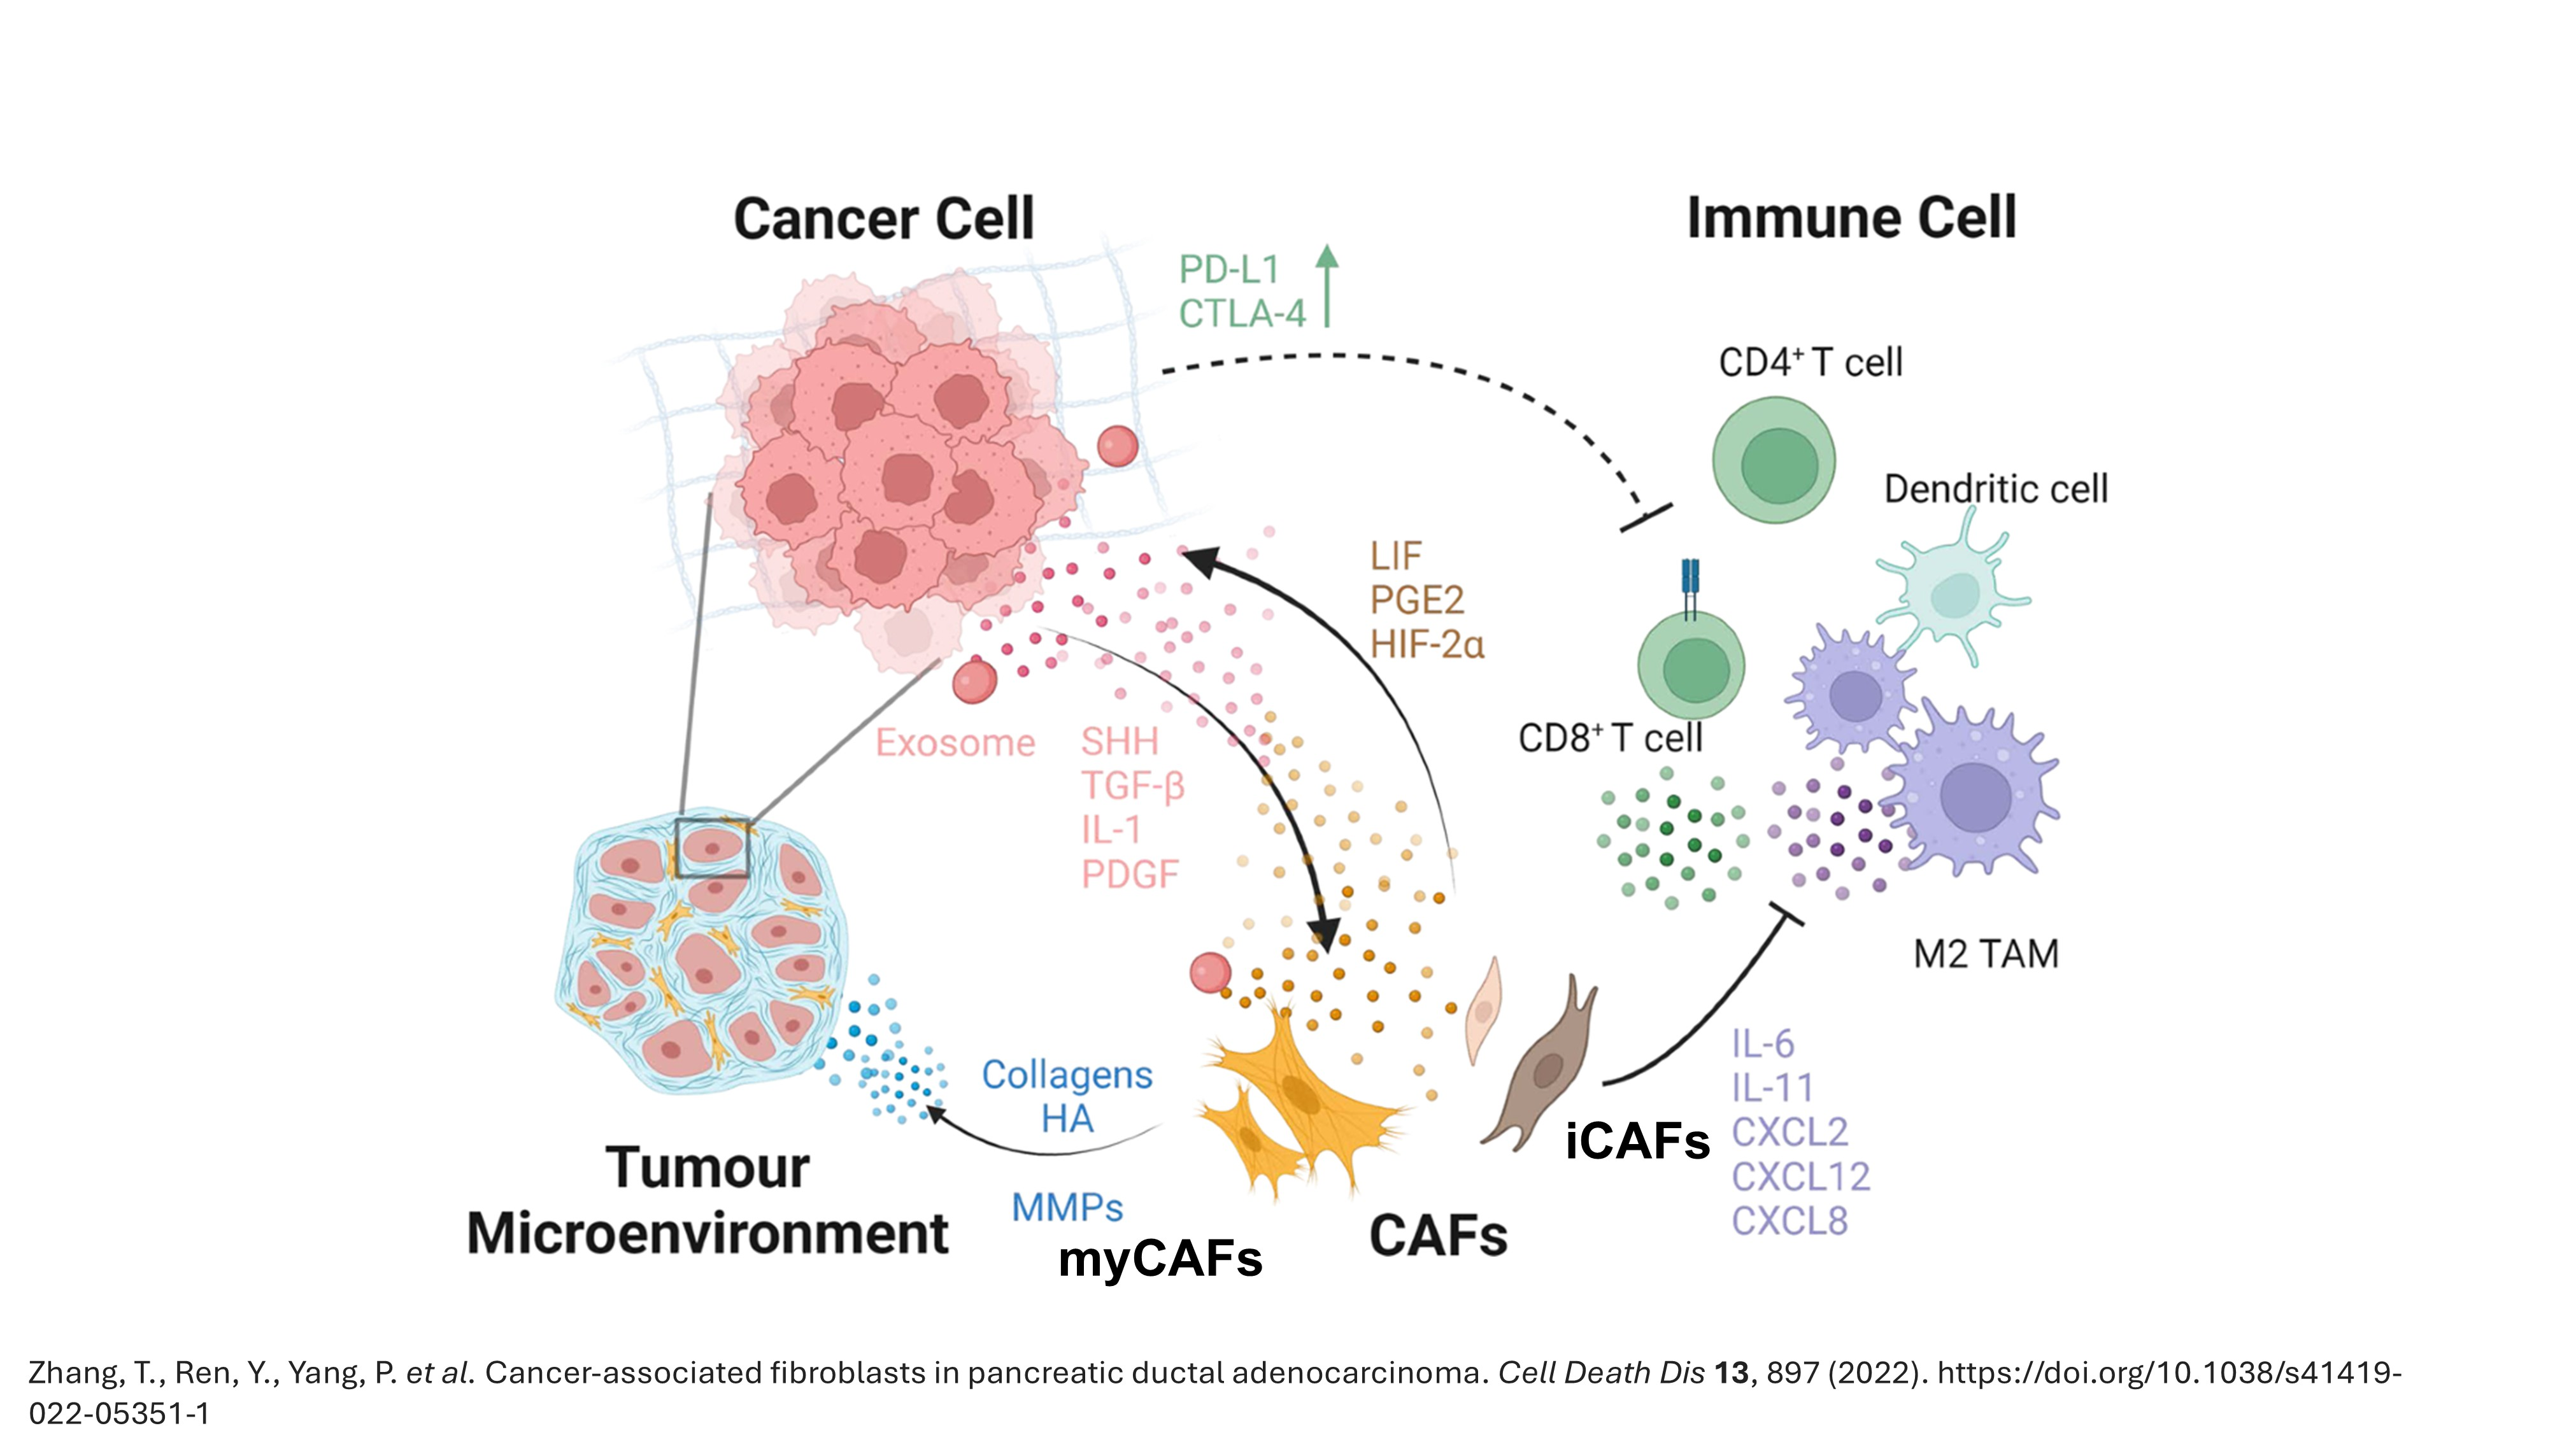
\includegraphics[width=1.05\textwidth]{F1.JPG}}
\caption{\textbf{Biological context of the PDAC stromal microenvironment.} PDAC epithelial cells are embedded in a dense stromal microenvironment structured by fibroblast heterogeneity, extracellular matrix remodeling, and immune interactions. The scheme shows the myCAF/iCAF framework.}
\end{figure}

Pancreatic ductal adenocarcinoma (PDAC) is not only a disease of malignant epithelial cells. It is also a disease of tissue organization. One of its main features is a strong desmoplastic reaction in which tumor cells coexist with abundant extracellular matrix (ECM), immune cells, and heterogeneous fibroblasts. This stromal compartment, meaning the non-malignant supportive tissue surrounding tumor cells, affects tumor growth, limits drug penetration, and shapes local immune regulation \citep{ohlund2017,elyada2019,oh2023}. For this reason, understanding stromal biology is important for understanding PDAC itself.

Cancer-associated fibroblasts (CAFs) are now recognized as a heterogeneous population rather than a single cell type. In PDAC, myofibroblastic CAFs (myCAFs) are usually described as matrix-rich and contractile, whereas inflammatory CAFs (iCAFs) are more secretory \citep{ohlund2017,elyada2019}. Recent single-cell studies also support the existence of more quiescent or resident-like stellate states and additional inflammatory or interferon-associated fibroblast programs \citep{hosein2019,oh2023}. In this report, this biological complexity is simplified into a practical contrast between an activated contractile stromal pole and a more quiescent resident-like stromal pole.

Previous work from the laboratory supports the idea that ion channels are not only passive markers in PDAC, but can actively participate in tumor/stroma communication. In particular, SK2 was shown to respond to CAF-derived signals and to reinforce signaling pathways associated with invasiveness and metastasis \citep{rapetti2023}.

So ion channels are relevant in this context because they regulate membrane potential, calcium entry, secretion, cell volume, and mechanical responses. In fibroblasts, these functions can influence contraction, matrix deposition, and communication with neighboring cells. However, ion channels are often expressed at relatively low transcript levels, especially in sparse single-cell or spatial assays, which makes them easy to miss if analysis relies only on absolute expression. This does not mean that they are biologically unimportant. A limited number of ion channels can still produce strong electrophysiological effects on membrane potential and calcium signaling, and these effects can translate into major functional changes \citep{scruggs2020,jiang2019}. In this project, I focused on the potassium channel family because it is the largest ion channel family and because potassium channel biology is a clear area of interest in the host laboratory.

The broader project initially identified a union of 25 KCN candidates across the stromal discovery analyses. Because this report is limited in size and number of figures, I focus on three genes that best structure the story. \textit{KCNMA1}, which encodes the pore-forming subunit of the BKCa channel, is used as the main activated stromal candidate. \textit{KCNJ8} is used as a candidate associated with a more quiescent or resident stromal pole. \textit{KCNN4} is used as a tumor epithelial counterpoint that helps distinguish stromal and epithelial territories. This tumor-oriented reading of \textit{KCNN4} is also consistent with PDAC literature, where \textit{KCNN4}-mediated signaling has already been linked to tumor progression \citep{jiang2019}. Other KCN genes remain interesting and will be discussed briefly in the final schematic and perspectives.

\section{Objectives}
The main objective of this internship was to identify ion channels that may modulate extracellular matrix organization and/or immune-related stromal functions in PDAC. To address this question, the report followed four linked goals. First, I sought to prioritize stromal potassium channel candidates in a stromal scRNA-seq dataset. Second, the focus shifted to validating and repositioning these candidates in a broader PDAC snRNA-seq atlas containing both stromal and tumor compartments. Third, I set out to test whether BKCa silencing in CAFs is associated with coherent transcriptomic changes. Fourth, the final step involved placing the main candidates back into tissue space using spot-based spatial transcriptomics. The ultimate goal was to build a coherent and readable stromal-centered interpretation supported by several data layers.

\section{Materials and Methods}

\subsection{Overall Bioinformatic Workflow}
This work is presented as a workflow rather than as a finalized pipeline. It combines four analytical blocks that match the main figures of the report: stromal single-cell prioritization, external validation in a broader snRNA-seq atlas, local bulk RNA-seq perturbation around BKCa signaling, and spatial transcriptomic localization. The workflow is currently being reorganized into a more reusable pipeline for later use in the project, in line with current practical single-cell analysis frameworks \citep{luecken2019,he2022}.

The project relied mainly on \textbf{R} and \textbf{Python} for data processing, statistical analysis, and figure generation. The main R packages were \texttt{Seurat} (single-cell analysis framework), \texttt{DESeq2} (count-based differential expression for RNA-seq), \texttt{MAST} (single-cell hurdle-model differential expression), \texttt{fgsea} (fast gene set enrichment analysis), \texttt{msigdbr}, \texttt{escape}, \texttt{ggplot2}, \texttt{ggrepel}, \texttt{VennDiagram}, \texttt{pheatmap}, and standard data-handling packages such as \texttt{dplyr} and \texttt{tibble}. The main Python packages were \texttt{scanpy} (single-cell analysis toolkit), \texttt{pandas}, and the \texttt{Hotspot} framework. All analyses performed during this internship are available in the GitHub repository \href{https://github.com/ym22000/pdac-ion-channels-m1}{ym22000/pdac-ion-channels-m1}.

\subsection{Moffitt Stromal scRNA-seq Discovery Block}
The first analytical block used a stromal Seurat object derived from the coordinated single-cell PDAC resource from Oh et al. \citep{oh2023}. ScRNA-seq measures the transcriptome of individual whole cells after dissociation. The full atlas contains several compartments, including tumor, immune, endothelial, and stromal populations, but the report starts from the stromal object because the focus is stromal. A broader tumor/stroma comparison was addressed later with the USER atlas, which is more suitable for that purpose.

The stromal object contained 21,469 stromal cells from 40 samples and 29 patients, distributed across eight stromal cell types. UMAP plots were read from the Seurat object and are based on normalized single-cell expression values. The object also contained the original activated-stroma and normal-stroma scores from the Moffitt framework. I used the difference between these two scores to define a broad \texttt{StromaState} variable. This was useful because it allowed the Venn diagram to include both the original activated/normal stromal view and finer subtype-specific contrasts.

Four complementary differential expression strategies were combined in Fig.~2b. Test 1 was a patient-aware pseudobulk \texttt{DESeq2} comparison between activated and normal like stromal states. In this test, raw counts were aggregated by patient and state before running a count-based negative binomial model with a Wald test \citep{love2014}. Test 2 was a patient-aware pseudobulk \texttt{DESeq2} subtype/rest comparison, again using aggregated raw counts. Test 3 was a cell-level hurdle model designed to separate gene detection from positive-expression behavior. Such models are useful in zero-inflated data because a gene can differ either by being detected more often or by being more strongly expressed when detected \citep{finak2015}. Test 4 was a standard \texttt{MAST} analysis using log-normalized single-cell expression values \citep{finak2015}. The Venn diagram therefore summarizes convergence across different input matrices and different statistical assumptions, which is important because single-cell results can vary substantially with analysis choices \citep{vieth2019}.

For the direct qPSC/myCAF comparison shown in Fig.~2d, raw counts were aggregated into patient-aware pseudobulk samples. Only paired patients with enough cells in both subtypes were retained, leading to 29 paired patients, 5,386 qPSC cells, and 4,699 myCAF cells. \texttt{DESeq2} was run with the design \texttt{\textasciitilde{} patient + subtype}. Hallmark gene set enrichment analysis (GSEA) was then performed with \texttt{fgsea} using the Wald statistic ranking \citep{subramanian2005,korotkevich2021}.

\subsection{USER snRNA-seq Validation Block}
The second analytical block used a broader PDAC single-nucleus RNA sequencing (snRNA-seq) dataset from Hwang et al. \citep{peng2020}. snRNA-seq measures nuclear RNA instead of whole-cell RNA and is often more stable in fibrotic tissues. In this report, this dataset is called the USER dataset. The key advantage of this dataset is that it contains the full microenvironment rather than fibroblasts alone, which makes it useful for placing stromal candidates back into a tumor/stroma context.

The global USER figure was built from published metadata and UMAP coordinates. The dataset contained 88,031 nuclei, including 17,537 fibroblast nuclei. The proportions of tumor and fibroblast nuclei varied noticeably across patients. This heterogeneity needed to be made explicit before performing the tumor/fibroblast comparison shown in Fig.~3b.

So for the tumor/fibroblast contrast, raw counts were aggregated by patient and cell subset. Only patients containing both tumor and fibroblast nuclei were kept. Genes with very low total counts were removed before analysis. \texttt{DESeq2} was then run with the design \texttt{\textasciitilde{} patient + group}. The final contrast included 15 paired patients, 43,817 tumor nuclei, 17,537 fibroblast nuclei, and 18,993 tested genes.
Also, differential expression analyses were performed across the broader set of major USER cell subsets, but are not detailed here because the tumor/fibroblast contrast is the most directly informative for repositioning stromal KCN candidates.

\subsection{Bulk RNA-seq Analysis of BKCa Silencing in CAFs}
The third analytical block used a local bulk RNA-seq dataset generated in the host laboratory. In this experiment, BKCa was silenced by short-hairpin RNA in cultured human CAFs, creating a \texttt{shBKCa} condition compared with non-targeting controls. In this report, BKCa refers to the large-conductance calcium-activated potassium channel complex centered on the pore-forming \textit{KCNMA1} gene and the associated beta-subunit genes \textit{KCNMB1} and \textit{KCNMB4}. Bulk RNA-seq measures the average transcriptome of each sample rather than individual cells. The comparison included four control samples and four \texttt{shBKCa} samples, and gene-level counts were collapsed into 17,889 genes.

Principal component analysis (PCA) was used as an internal quality control step on normalized transformed expression values to confirm separation of replicates by condition, although this PCA is not shown here. Differential expression was performed on raw count data with \texttt{DESeq2} \citep{love2014}. Hallmark pathway enrichment was performed with \texttt{fgsea}, using the gene-level log2FC ranking and following the general GSEA framework \citep{subramanian2005,korotkevich2021}. CAF signature heatmaps were built from normalized expression values scaled by gene across samples, corresponding in the legend to a row z-score. At signature level, condition differences were summarized with Wilcoxon rank-sum tests. The myCAF and iCAF signatures were based on published PDAC CAF states, from Ohlund et al. and Elyada et al. \citep{ohlund2017,elyada2019}.

\subsection{Spatial Transcriptomics and Signature Projection}
The spatial block used a Visium FFPE PDAC dataset from Khaliq et al. \citep{khaliq2024}. Spatial transcriptomics measures RNA expression at spot level while preserving tissue coordinates. In this dataset, the 30 tissue sections represented 91,496 spots in total, including 3 normal pancreas sections (9,820 spots), 10 PDAC sections (35,458 spots), 12 liver metastasis sections (28,520 spots), and 5 lymph node sections (17,698 spots). Structural annotations and multicellular ecotypes from the reference study were reused as a tissue framework.

I focused mainly on normal pancreas and primary PDAC sections because the focus concerns pancreatic stromal organization. Liver metastasis and lymph node sections remain useful in the larger project, but they are not necessary to support the  argument developed here.

Spatial interpretation relied on two complementary levels. First, local Hotspot maps were used to visualize spatially coherent territories for \textit{KCNMA1} and \textit{KCNN4}. \texttt{Hotspot} framework detects locally structured patterns rather than isolated high spots, which makes it useful for distinguishing real tissue territories from scattered signal \citep{detomaso2021}. Second, reference signatures were projected at spot level and compared with KCN signals using Spearman rank correlation. Spearman correlation was preferred because spot-level values are sparse, non-gaussian, and better interpreted through monotonic association than strict linearity.

The tumor epithelial signature used in Fig.~6a was defined in the laboratory from epithelial markers considered informative in this project (\textit{EPCAM}, \textit{MUC1}, \textit{KRT7}, \textit{KRT8} and \textit{KRT18}). The CAF signature used in Fig.~6b came from the reference spatial study and was projected as a paper-derived ssGSEA-like score \citep{khaliq2024}. In practice, the spatial analysis combined R and Python processing using \texttt{Seurat}, \texttt{escape}, \texttt{scanpy}, \texttt{pandas}, and \texttt{Hotspot}.

\subsection{Statistics and Multiple Testing}
Effect size is mainly described in this report with log2FC, and statistical significance is summarized with adjusted p-values or false discovery rate (FDR). In \texttt{DESeq2}, p-values came from Wald tests on count-based negative binomial models \citep{love2014}. In \texttt{MAST}, p-values came from a hurdle framework applied to log-normalized expression \citep{finak2015}. Because omics analyses test many genes and pathways at the same time, multiple testing correction was performed with the Benjamini-Hochberg (BH) method rather than Bonferroni correction. BH was preferred because it controls the expected proportion of false discoveries while preserving reasonable sensitivity in discovery oriented transcriptomic analyses.

Single-cell and single-nucleus differential results were interpreted together with pseudobulk analyses to avoid over-reliance on cell-level pseudoreplication. Wilcoxon tests were used for non-parametric comparison of summary scores, such as CAF signatures in bulk RNA-seq. Spearman correlation was used in the spatial block for spot-level association analyses.

\section{Results and Discussion}

\subsection{A Stromal KCN Core Was Identified in the Moffitt Dataset}
\begin{figure}[H]
\centering
\makebox[\textwidth][c]{
\includegraphics[width=0.94\textwidth]{F2.png}}
\caption{\textbf{Stromal single-cell prioritization in the Moffitt dataset.} \textbf{a} UMAP representation of stromal cell subtypes. \textbf{b} Four-test Venn summary showing overlap between complementary differential expression strategies used to prioritize KCN candidates across cell-level and pseudobulk approaches. \textbf{c} Volcano plots from the pseudobulk subtype/rest analysis highlighting KCN behavior across stromal subtypes. \textbf{d} Hallmark GSEA comparison between qPSC and myCAF.}
\end{figure}

In this section, as shown in Fig.~2a, the stromal compartment is not a homogeneous fibroblast cloud. It is organized into qPSC, smPSC, myCAF, csCAF, and iCAF states, together with smaller associated populations. This matters because the project question is not only whether a KCN gene is stromal, but also which stromal state it follows. The stromal object contained 21,469 cells in total, including 5,743 qPSCs, 5,521 smPSCs, 4,809 myCAFs, 4,242 csCAFs, and only 338 iCAFs.

As shown in Fig.~2b, the four differential expression strategies converge on a compact robust core. The full union of candidates was useful to preserve potentially relevant KCN genes at an exploratory stage, but the strict intersection is the most robust part of the result. Nine KCN genes were detected by all four methods (\textit{KCNA5}, \textit{KCNAB1}, \textit{KCNC4}, \textit{KCND3}, \textit{KCNE4}, \textit{KCNJ8}, \textit{KCNK17}, \textit{KCNK6}, and \textit{KCNMA1}). This convergence is important because the four methods do not test exactly the same thing. The two pseudobulk tests are conservative and sample-aware. The hurdle-based single-cell tests (Test 3 and 4) are more sensitive to sparse detection behavior. The \texttt{StromaState} comparison was also worth keeping because it reconnects the subtype-based analysis to the original activated/normal stromal logic from the Moffitt framework.

As shown in Fig.~2c, the subtype-specific effect sizes refine this convergence. In the pseudobulk subtype/rest analysis, \textit{KCNMA1} was strongly enriched in smPSC with log2FC = 3.73 (FDR = $1.30\times 10^{-10}$) and was also enriched in myCAF with log2FC = 2.00 (FDR = $3.63\times 10^{-3}$). In contrast, \textit{KCNJ8} was enriched in qPSC with log2FC = 1.67 (FDR = $9.11\times 10^{-7}$) and strongly depleted in myCAF with log2FC = -3.16 (FDR = $4.04\times 10^{-11}$). \textit{KCNN4} did not emerge as a significant stromal subtype marker in this stromal setting. These values align with the primary stromal polarity established in this report, wherein \textit{KCNMA1} delineates an activated, contractile pole, whereas \textit{KCNJ8} characterizes a more quiescent, resident-like phenotype.

As shown in Fig.~2d, this polarity is not limited to single genes. The myCAF side is enriched in epithelial-mesenchymal transition, TGF-$\beta$ signaling, coagulation, hypoxia, glycolysis, and KRAS signaling up. In contrast, qPSC is enriched in oxidative phosphorylation, fatty acid metabolism, interferon response, and DNA repair. The iCAF axis was explored, but it remained less robust in this dataset. This is consistent with the low number of iCAF cells. For example, \textit{KCNJ8} showed log2FC = -3.34 in iCAF but remained non-significant after correction (FDR = 0.311), and \textit{KCNMA1} showed a modest positive signal without significance. In this report, iCAF is therefore treated as an explored but unresolved axis rather than as a fourth strong KCN-centered pole.

\subsection{USER Validation Repositioned the Candidates Along a Tumor--Stroma Axis}
\begin{figure}[H]
\centering
\makebox[\textwidth][c]{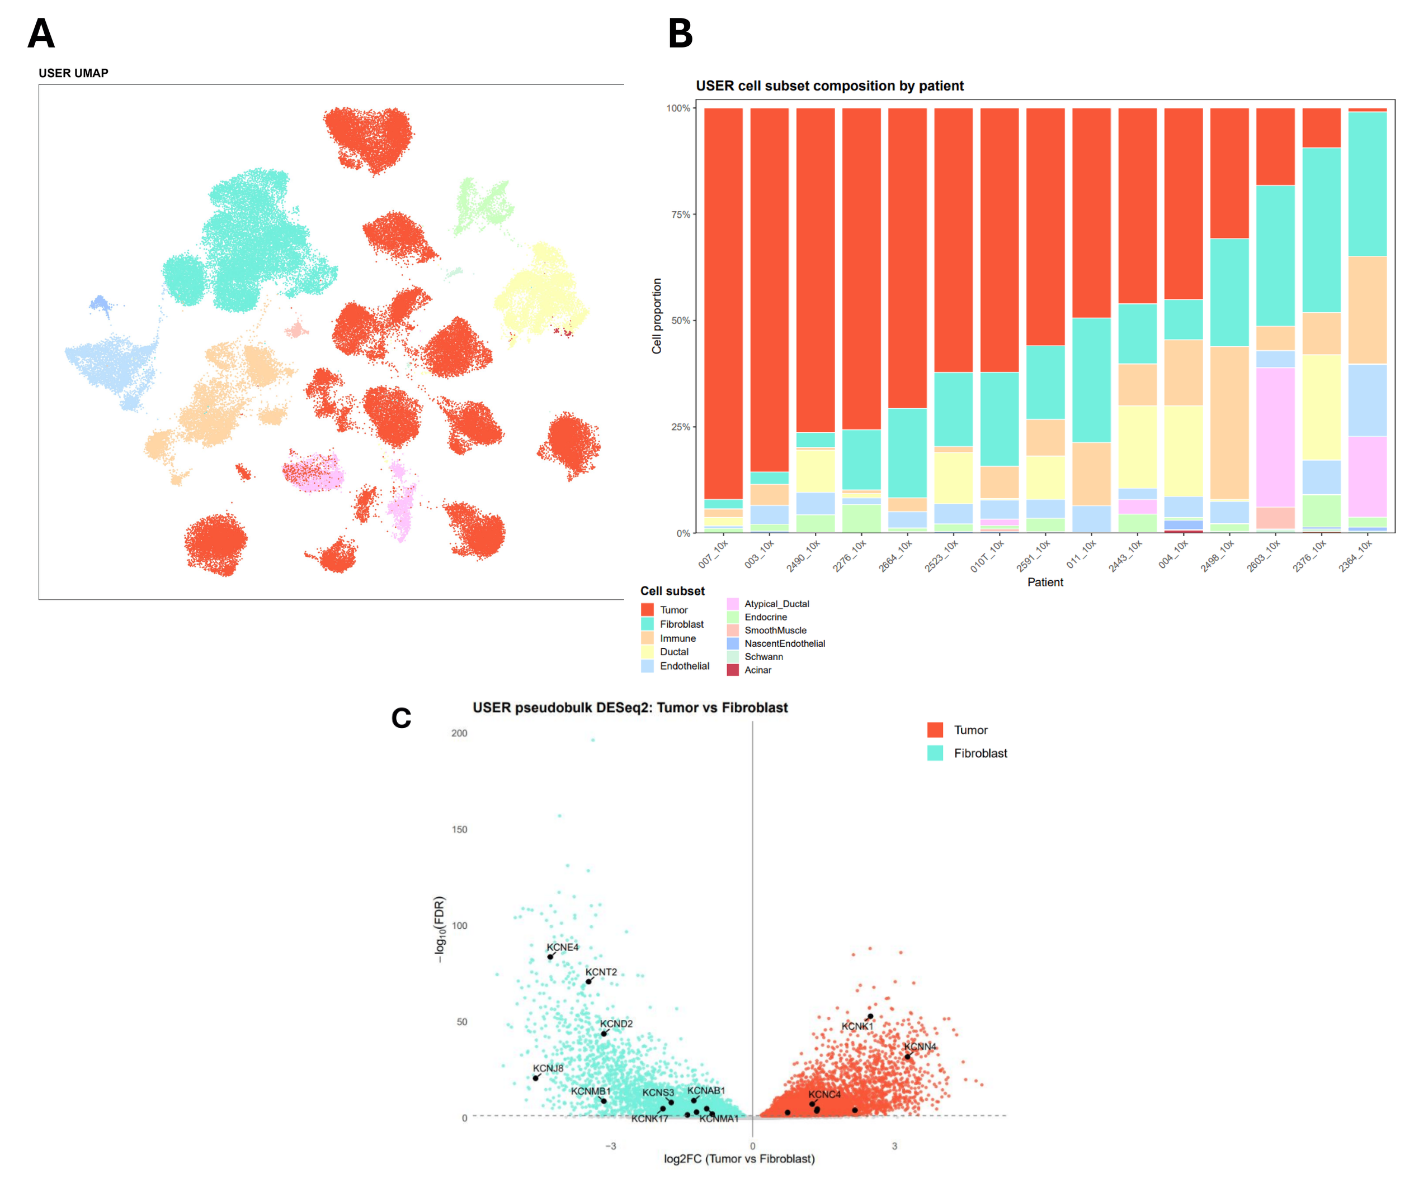
\includegraphics[width=1.0\textwidth]{F3.png}}
\caption{\textbf{External validation in the USER snRNA-seq dataset.} \textbf{a} UMAP of the USER PDAC atlas used to reinsert stromal candidates into a broader tumor microenvironment context. \textbf{b} Cell-type composition across patients, shown to highlight inter-patient variability and to justify patient-aware pseudobulk analyses. \textbf{c} Volcano plot of the pseudobulk Tumor/Fibroblast comparison, used to position the selected KCN candidates along a stromal/tumor axis.}
\end{figure}

In this section, as shown in Fig.~3a, the candidates are repositioned in a broader whole-tissue context. This is important because a gene that looks stromal inside a fibroblast object can still be shared with other compartments when the whole tumor microenvironment is considered. The USER atlas is particularly useful for this because it contains tumor, fibroblast, immune, endothelial, and ductal compartments in the same framework.

As shown in Fig.~3b, there is strong inter-patient variation in cellular composition. Some samples are largely tumor-dominated, whereas others contain larger fibroblast fractions. This justifies the patient-aware pseudobulk design used for the tumor/fibroblast contrast. Without this design, large patient-specific composition effects could be mistaken for true gene-specific biology.

A volcano plot summarizes differential expression by showing effect size on the x-axis and statistical significance on the y-axis. As shown in Fig.~3c, the simplest global question is whether a gene is closer to tumor or fibroblast in the full atlas. In this direct Tumor/Fibroblast comparison, \textit{KCNN4} was strongly tumor-up, with log2FC = 3.27 and FDR = $1.23\times 10^{-32}$. In contrast, \textit{KCNJ8} was strongly fibroblast-up, with log2FC = -4.59 and FDR = $1.92\times 10^{-21}$. \textit{KCNMA1} also remained on the fibroblast side, with log2FC = -0.975 and FDR = $1.13\times 10^{-5}$, although the effect size was smaller than for \textit{KCNJ8}. This result is informative for the general model. It confirms \textit{KCNN4} as a tumor epithelial counterpoint, keeps \textit{KCNJ8} as a strongly fibroblast-oriented gene, and places \textit{KCNMA1} in a stromal-centered but more microenvironmental position. This validation is also coherent with the Moffitt prioritization, because \textit{KCNJ8} and \textit{KCNMA1} belonged to the robust 4/4 core, whereas \textit{KCNN4} emerged in only 2 of the 4 DEG strategies.

\subsection{BKCa Knockdown in CAFs Altered Programs Linked to Activated Stroma}
\begin{figure}[H]
\centering
\makebox[\textwidth][c]{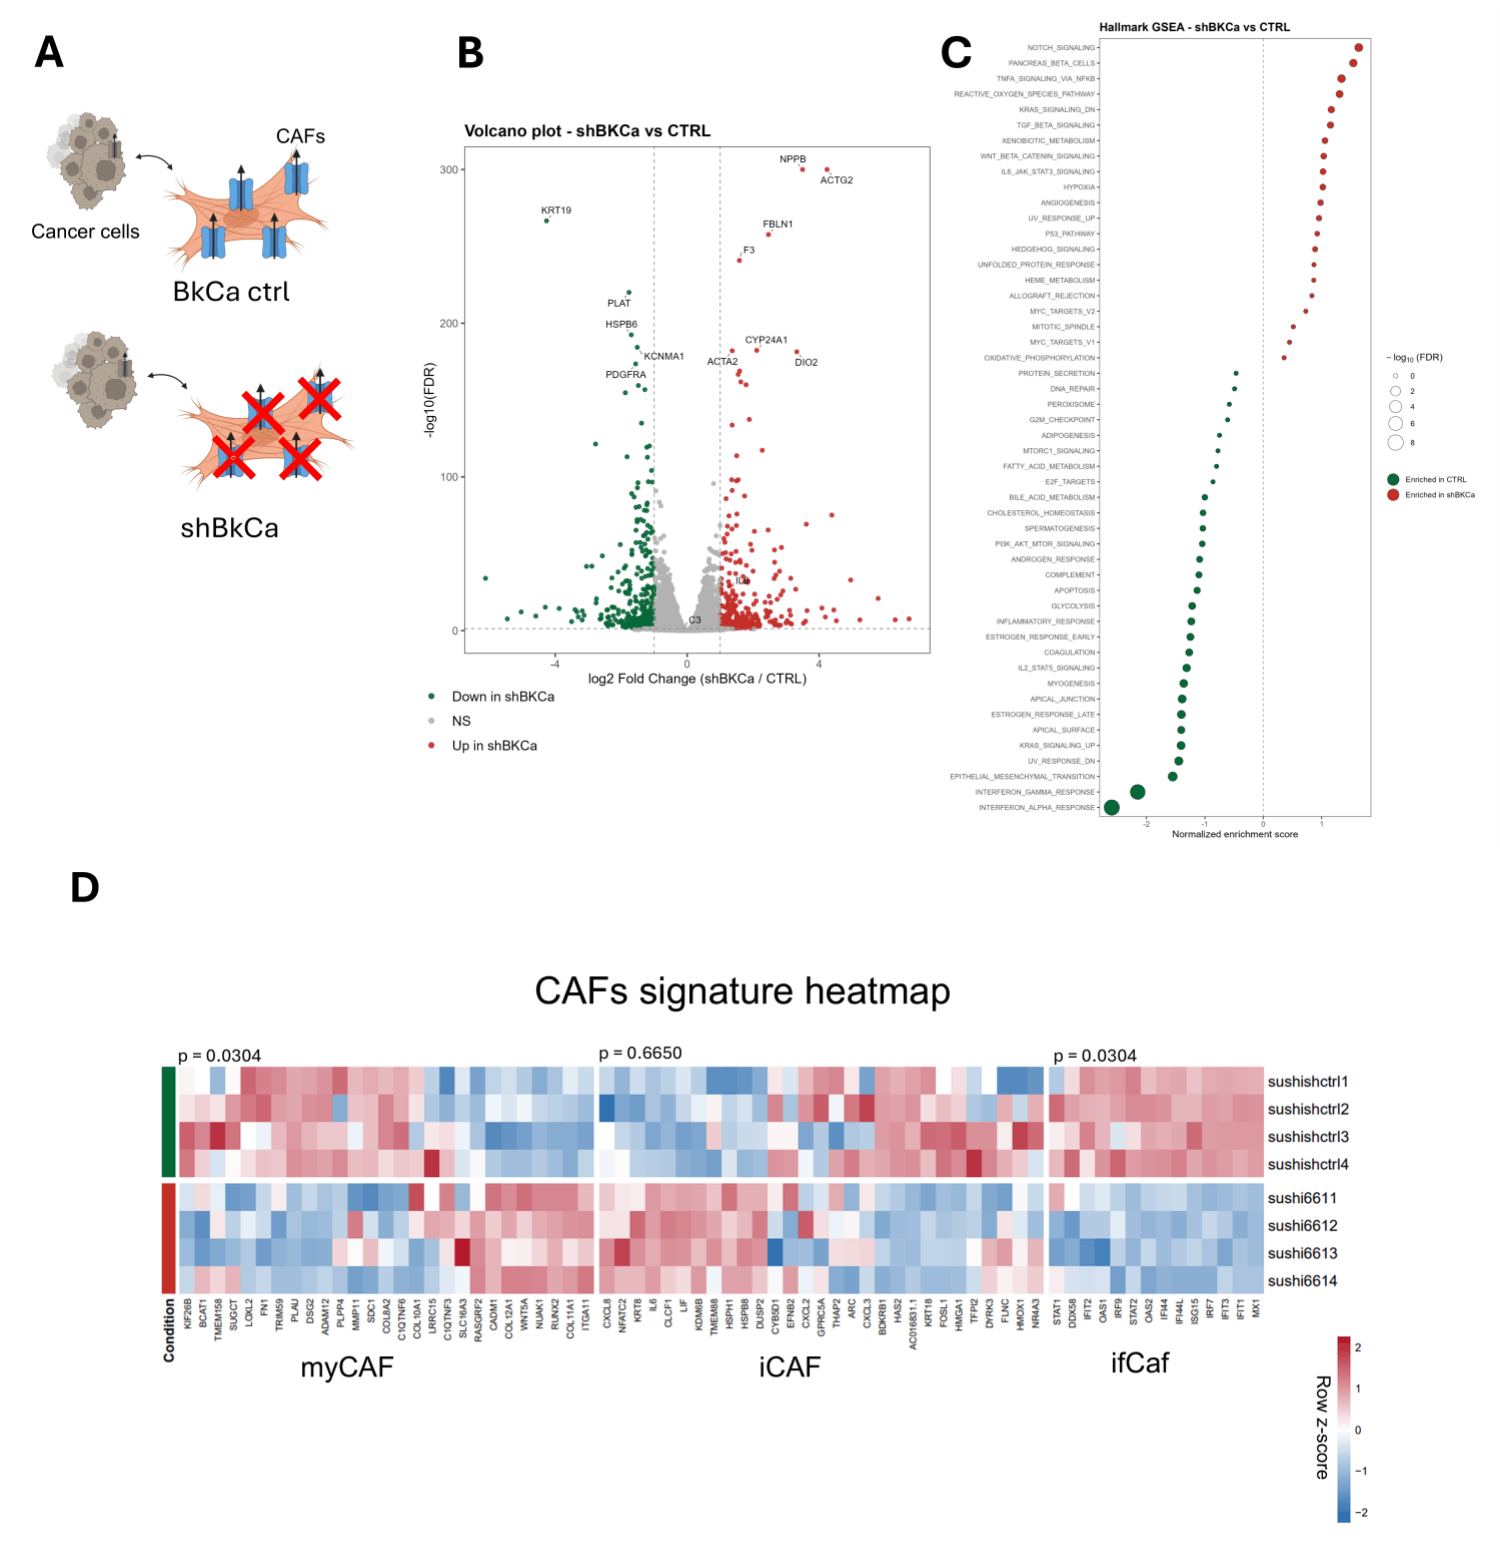
\includegraphics[width=1.05\textwidth]{F4.png}}
\caption{\textbf{Bulk RNA-seq perturbation analysis in a BKCa-centered CAF model.} \textbf{a} Experimental overview of the control and shBKCa comparison used in the local bulk RNA-seq block. \textbf{b} Volcano plot of differential expression between shBKCa and control samples. \textbf{c} Hallmark GSEA summary used to identify broad transcriptomic programs associated with the perturbation. \textbf{d} Heatmap of selected CAF-related signatures, including myCAF, iCAF, and ifCAF related markers, used to examine whether the perturbation is associated with stromal program shifts.}
\end{figure}

In this section, as shown in Fig.~4a, the question is no longer where a gene is expressed, but whether BKCa silencing in CAFs changes the transcriptome in a way. This part adds a functional layer from the host laboratory to the descriptive analyses.

As shown in Fig.~4b, the perturbation worked. \textit{KCNMA1} itself was reduced in \texttt{shBKCa}, with log2FC = -1.51 and FDR = $4.45\times 10^{-185}$. The volcano plot shows changes in structural or stromal genes such as \textit{ACTA2}, \textit{ACTG2}, \textit{FBLN1}, and \textit{PDGFRA}, supporting the idea that BKCa signaling is linked to stromal cell state.

At pathway level, as shown in Fig.~4c, the strongest significant enrichments are found on the control side, especially interferon alpha response, interferon gamma response, and epithelial-mesenchymal transition. In other words, the major effect of BKCa silencing in this model is not the appearance of one dominant new program, but rather the weakening of already structured programs.

As shown in Fig.~4d, the CAF heatmap is useful for the stromal interpretation because it suggests a global shift in CAF state rather than a single binary marker change. The clearest pattern is seen for the ifCAF signature, which is markedly lower in \texttt{shBKCa} than in controls (mean score 0.84 in CTRL / -0.84 in \texttt{shBKCa}; nominal Wilcoxon p = 0.0304, BH-adjusted FDR = 0.076). The myCAF signature also tends to decrease in \texttt{shBKCa} (mean score 0.12 in CTRL / -0.12 in \texttt{shBKCa}; p = 0.0304), but the heatmap indicates more heterogeneity across samples than for ifCAF. In contrast, the iCAF signature is more variable and does not show a robust directional shift (p = 0.665). Although limited by the small cohort size (n = 8), this pattern supports the idea that BKCa is not only associated with one CAF marker set, but more broadly acts as a driver of CAF signatures and CAF plasticity.

\subsection{Spatial Analyses Distinguished Stromal and Epithelial Territories}
\begin{figure}[H]
\centering
\makebox[\textwidth][c]{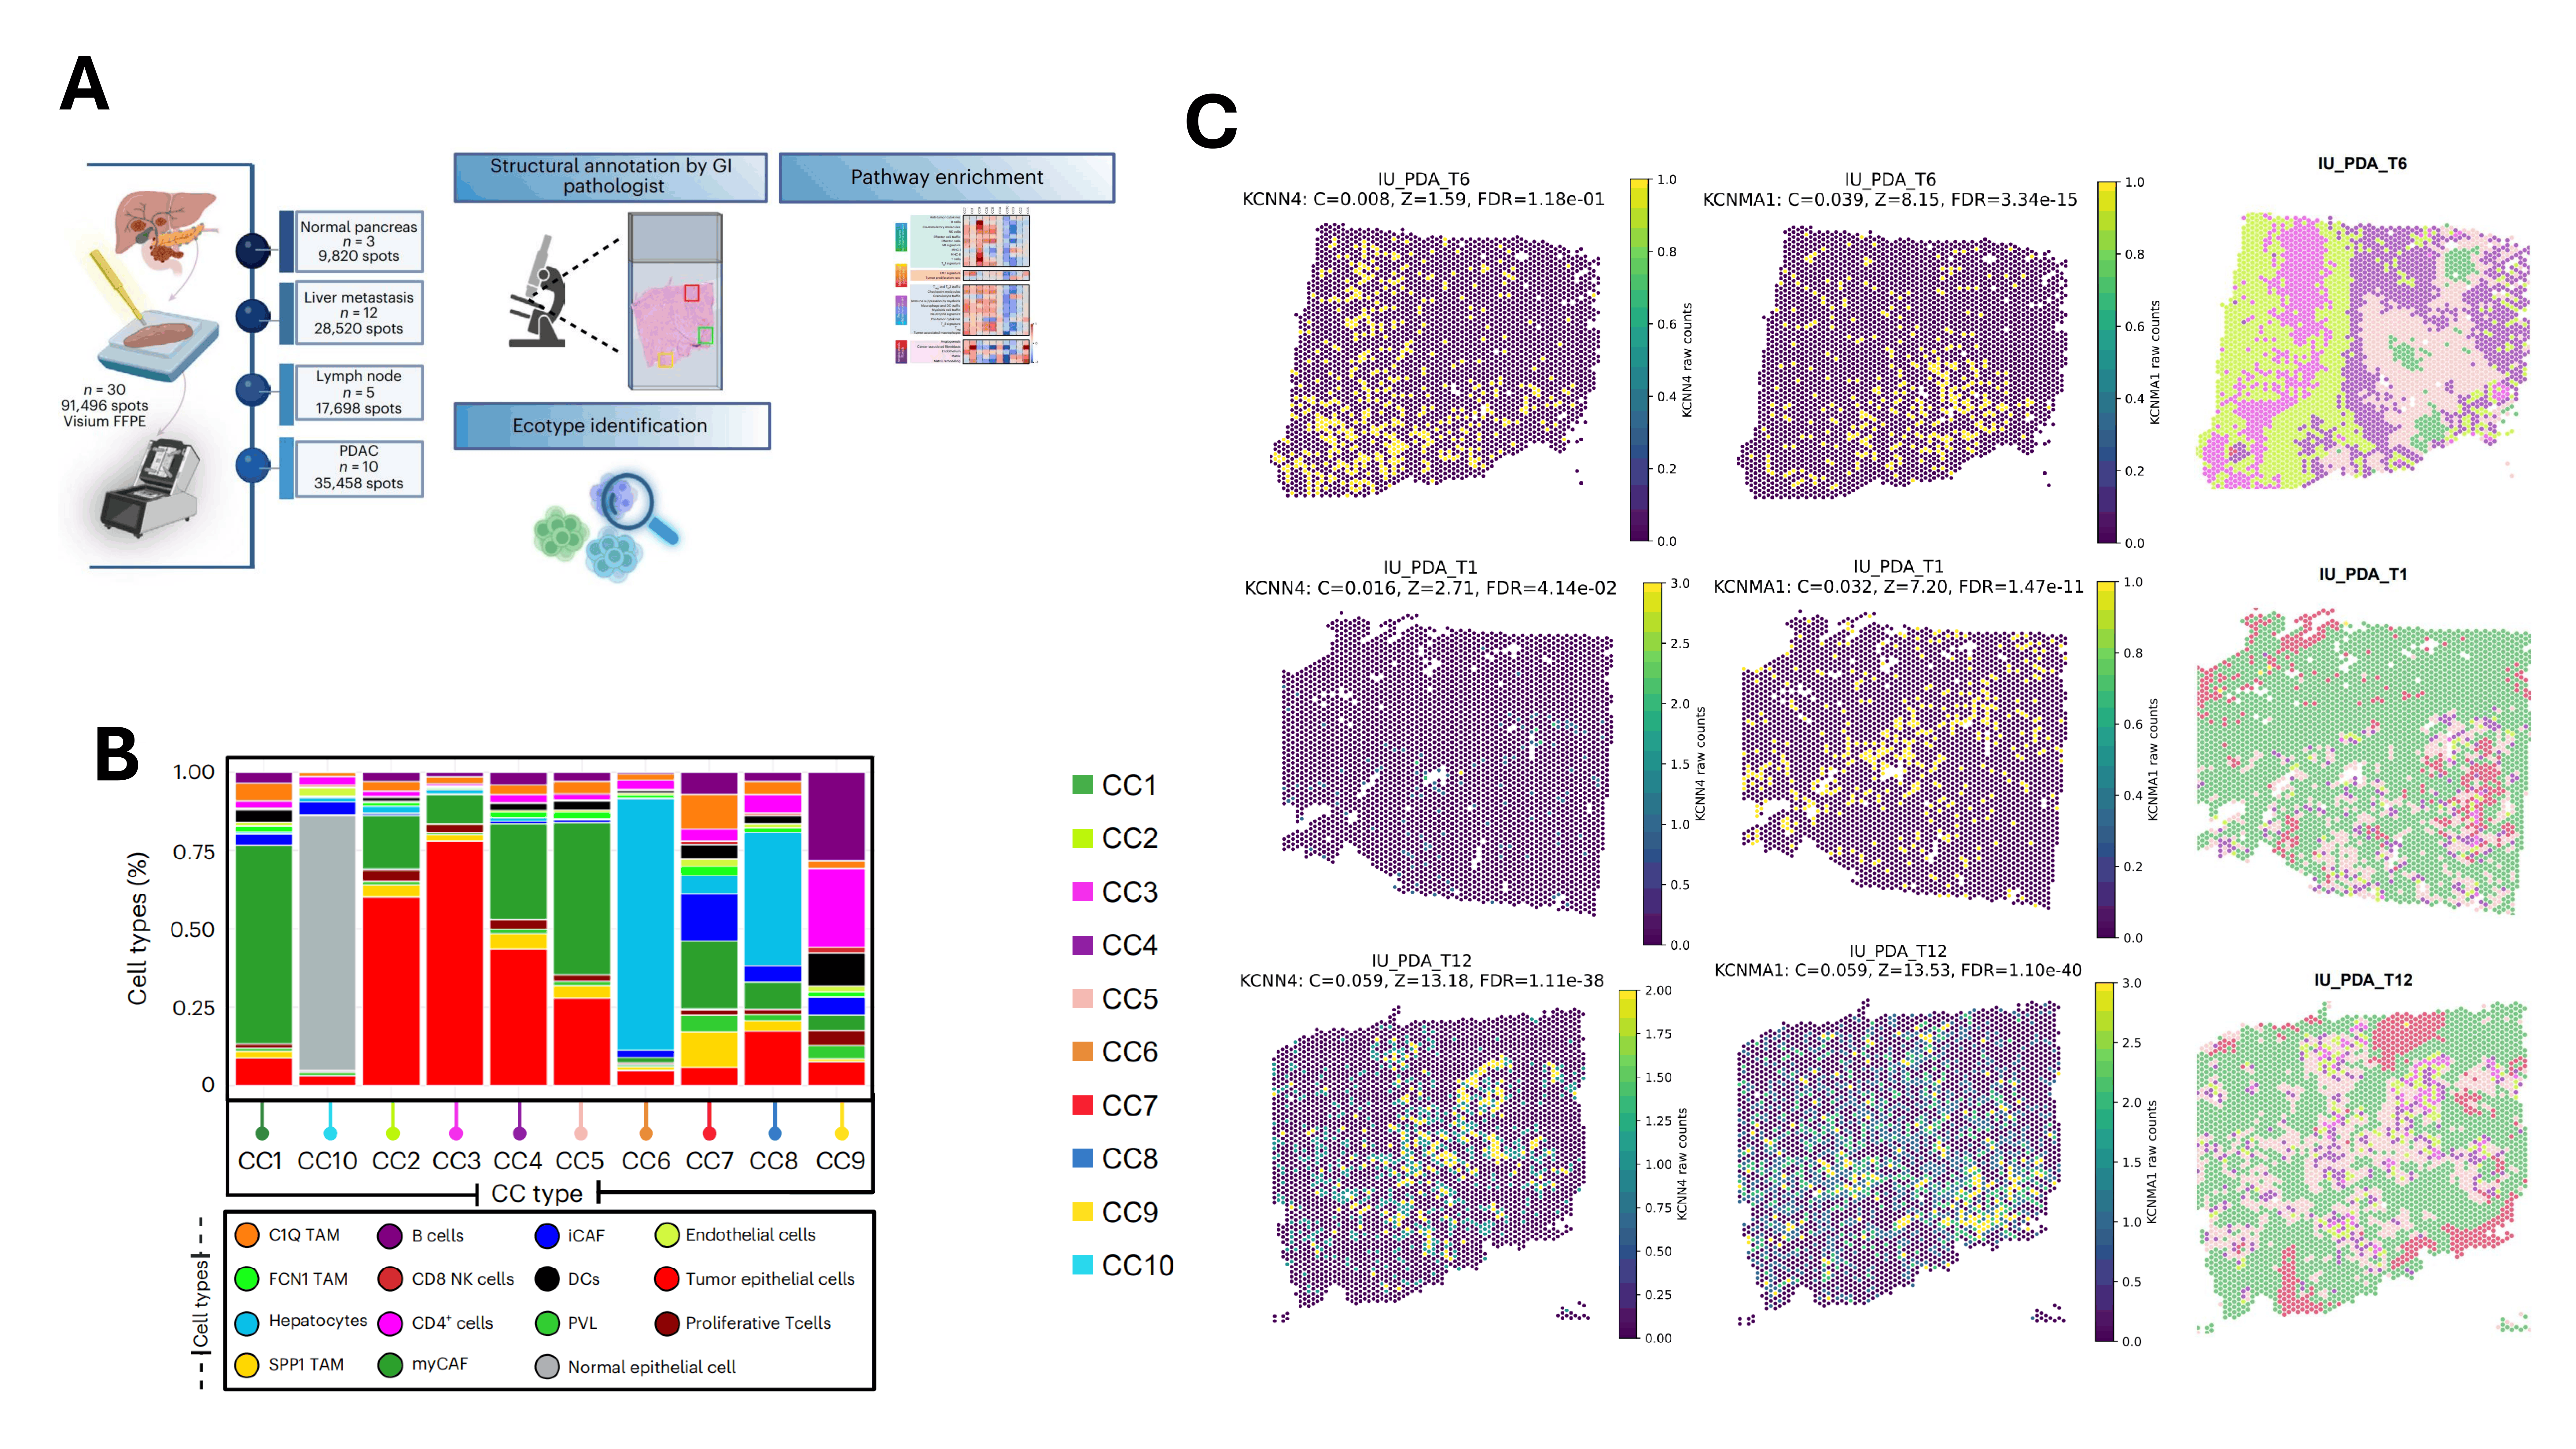
\includegraphics[width=1.08\textwidth]{F5.png}}
\caption{\textbf{Spatial transcriptomic context for the main KCN candidates.} \textbf{a} Overview of the spatial transcriptomic dataset, including section types, spot numbers, and ecotype information used. \textbf{b} Ecotype composition summary from the reference PDAC study. \textbf{c} Representative Hotspot maps for \textit{KCNMA1} and \textit{KCNN4} in selected PDAC sections (T6, T1, and T12), shown together with the neighboring ecotype context.}
\end{figure}

In this section, as shown in Fig.~5a, the analysis returns to tissue architecture. For the Hotspot results discussed in Fig.~5, the Z score corresponds to the standardized strength of spatial autocorrelation for a gene within one section, C is the associated scaled autocorrelation coefficient, and FDR is the Benjamini-Hochberg-adjusted significance of this spatial test. Higher positive Z and C values indicate a more coherent patch spatial pattern rather than diffuse expression. For the signature projections discussed in Fig.~6, $\rho$ denotes the Spearman rank correlation between a KCN gene and the projected signature across spots in one section \citep{detomaso2021}. The spatial dataset, as shown in Fig. 5a spans several anatomical contexts, but as said before, the report focuses mainly on normal pancreas and primary PDAC sections because these are relevant here. Fig. 5b recalls the multicellular ecotypes/niches described in the reference spatial study.

As shown in Fig.~5c, in T6, T1, and T12, \textit{KCNMA1} is repeatedly detected in regions compatible with stromal or mixed microenvironmental territories (ecotypes CC1 and CC5 in the paper), whereas \textit{KCNN4} is more dependent and visually closer to epithelial tumor territories (ecotypes CC2 and CC3). A complementary spot level Wilcoxon analysis across primary PDAC sections supported this interpretation. Therefore, the ecotype maps next to these panels help interpret these signals as territory associations rather than pure single-cell identities, because Visium spots average transcripts from small multicellular neighborhoods.

 Although it is not shown here, \textit{KCNJ8} displayed a stronger spatial Hotspot signal in normal pancreas than in primary PDAC, with a median Z score of 5.17 across normal sections / 1.15 across PDAC sections, together with a higher median C value (0.0238 / 0.00617). In the report, \textit{KCNJ8} is therefore mainly supported by the stromal polarity seen in Moffitt and confirmed in USER, while its spatial pattern also suggests relative enrichment in non-diseased pancreatic tissue compared with PDAC.

\subsection{Signature Projection Strengthened the Contrast Between KCNMA1 and KCNN4}
\begin{figure}[H]
\centering
\makebox[\textwidth][c]{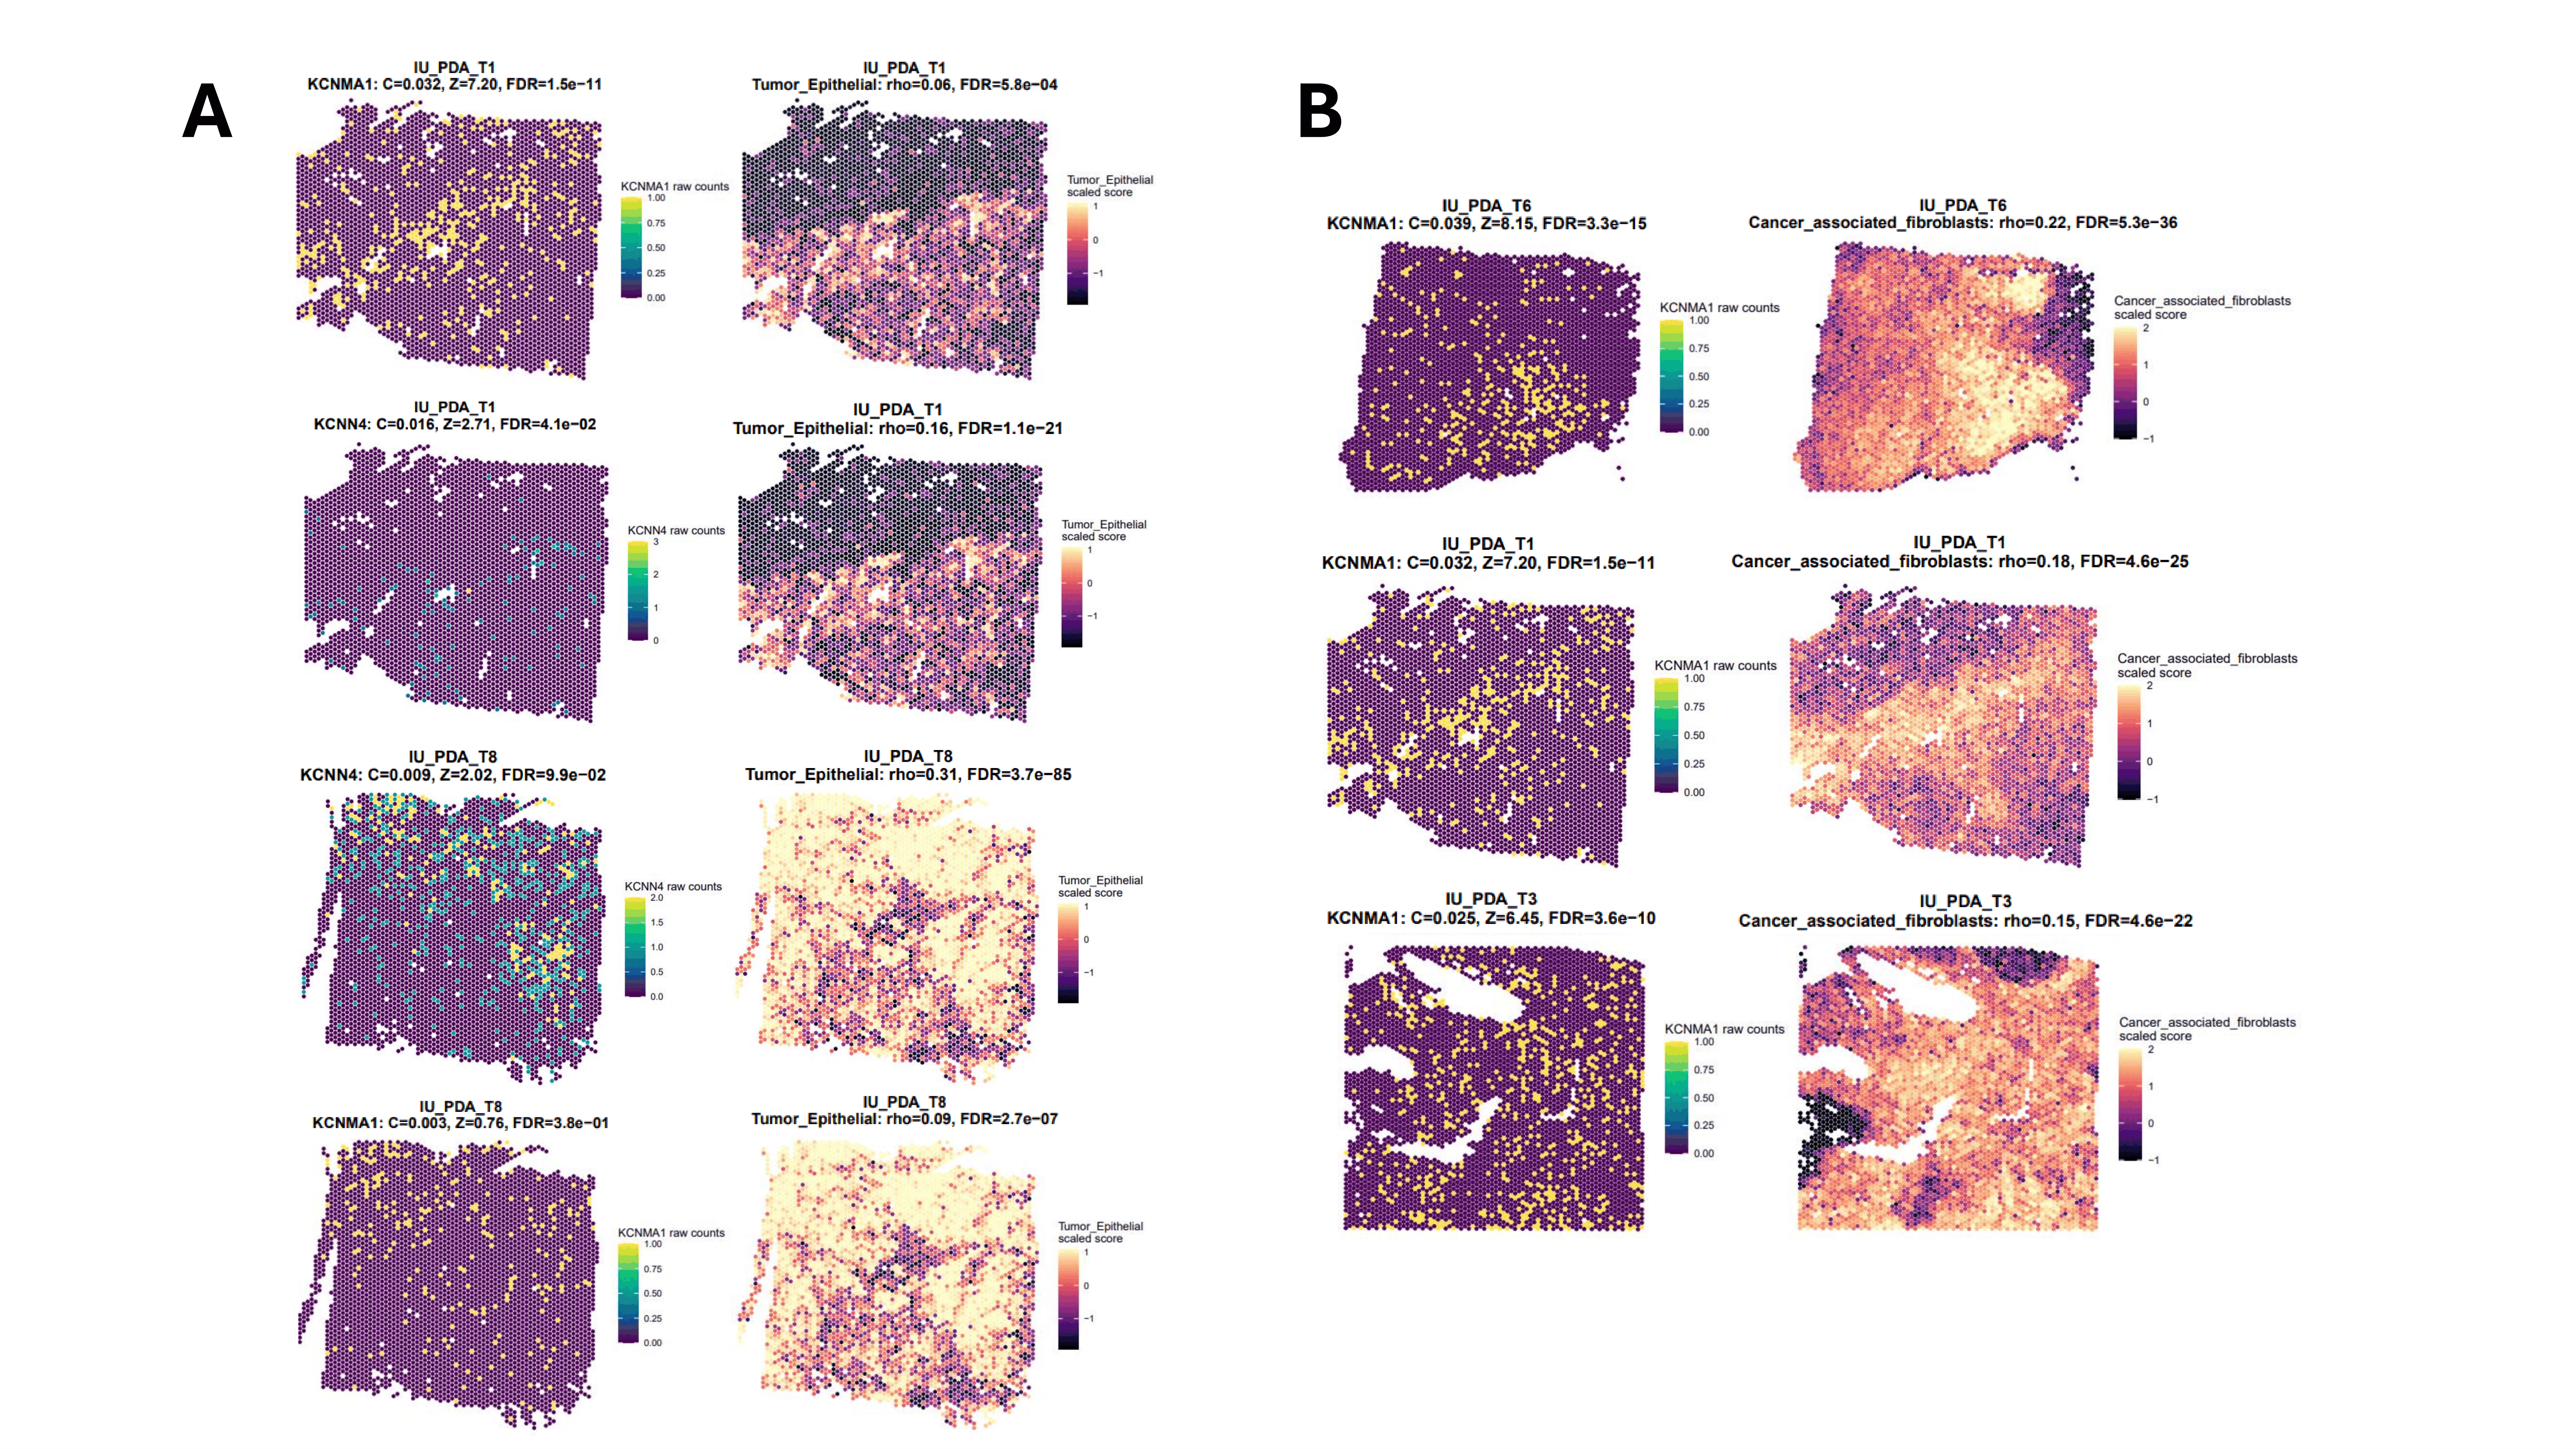
\includegraphics[width=1.08\textwidth]{F6.png}}
\caption{\textbf{Spatial projection of tumor epithelial and CAF-related signatures.} \textbf{a} Spot-level Spearman correlation projections comparing \textit{KCNMA1} and \textit{KCNN4} with a manually defined tumor epithelial signature in selected PDAC sections T1 and T8. \textbf{b} Spot-level comparison between \textit{KCNMA1} and the cancer-associated fibroblast score in representative sections T6, T1, and T3.}
\end{figure}

In this section, the spatial reading is refined by comparing gene expression to continuous biological signatures. This is because a spot-level gene map alone can remain ambiguous, whereas a spot-level correlation with a known reference program gives a more quantitative interpretation. This analysis was also motivated by the observation that \textit{KCNMA1} seemed to overlap with other spatial patterns that appeared more local than the ecotype structure.

As shown in Fig.~6a, \textit{KCNN4} follows the manually defined tumor epithelial signature more clearly than \textit{KCNMA1}. In T1, the tumor epithelial score correlated with \textit{KCNN4} at $\rho = 0.16$ (FDR = $1.1\times 10^{-21}$), whereas the correlation with \textit{KCNMA1} was lower at $\rho = 0.06$ (FDR = $5.8\times 10^{-4}$). In T8, the same trend remained visible, with $\rho = 0.31$ for \textit{KCNN4} (FDR = $3.7\times 10^{-85}$) and $\rho = 0.09$ for \textit{KCNMA1} (FDR = $2.7\times 10^{-7}$). These values are consistent with the USER tumor/fibroblast result and strengthen the interpretation of \textit{KCNN4} as a tumor epithelial counterpoint.

As shown in Fig.~6b, \textit{KCNMA1} provides the opposite information. Across the sections shown, \textit{KCNMA1} positively tracked the CAF score, with $\rho = 0.22$ in T6 (FDR = $5.3\times 10^{-36}$), $\rho = 0.18$ in T1 (FDR = $4.6\times 10^{-25}$), and $\rho = 0.15$ in T3 (FDR = $4.6\times 10^{-22}$). This does not imply exclusive expression in every fibroblast-containing spot, but it strongly supports a preferential association with stromal and CAF territories.

Taken these results together, \textit{KCNN4} is better aligned with tumor epithelial territories, whereas \textit{KCNMA1} is better aligned with stromal and CAF-rich territories. This spatial contrast completes the multi-level interpretation built from Moffitt, USER, and the local bulk perturbation model.

\subsection{Cross-Dataset Limits and Interpretation of Low Ion Channel Expression}
An important limitation of this project is that ion channels are often lowly expressed at transcript level across all the data types used here. This is true in scRNA-seq, where dropout and sparse counts reduce detection sensitivity; in snRNA-seq, where nuclear capture can underrepresent some transcripts; in bulk RNA-seq, where stromal signals are averaged across the whole sample; and in spatial transcriptomics, where spot-level averaging dilutes rare or localized signals. For this reason, absolute expression alone is not a sufficient criterion to evaluate the relevance of ion channels in PDAC.

Another limitation is that many ion channel genes are not only weakly expressed, but can also have several transcript variants. Therefore, 3'-biased scRNA-seq, snRNA-seq, and spatial methods are useful for gene-level detection, but less informative for transcript-level complexity.

This limitation is (especially) important for potassium channels because their biological importance does not scale linearly with transcript abundance. Even a modest number of channels can shift membrane potential, calcium entry, cell volume regulation, or contractile behavior. In fibroblasts and myofibroblasts, these functions can directly affect matrix remodeling and tissue mechanics \citep{scruggs2020}. In tumor cells, channels such as \textit{KCNN4} can support calcium-dependent signaling and tumor progression \citep{jiang2019}. In other words, low transcript abundance does not mean low functional significance.

This is why the workflow was built around convergence rather than single evidence. Instead of relying only on raw expression level, the project combined differential expression, patient-aware pseudobulk analysis, pathway association, perturbation response, and tissue localization. This does not remove all uncertainty, but it provides a more balanced way to study low-abundance but potentially high-impact genes.

\section{Conclusions and Perspectives}
\begin{figure}[H]
\centering
\makebox[\textwidth][c]{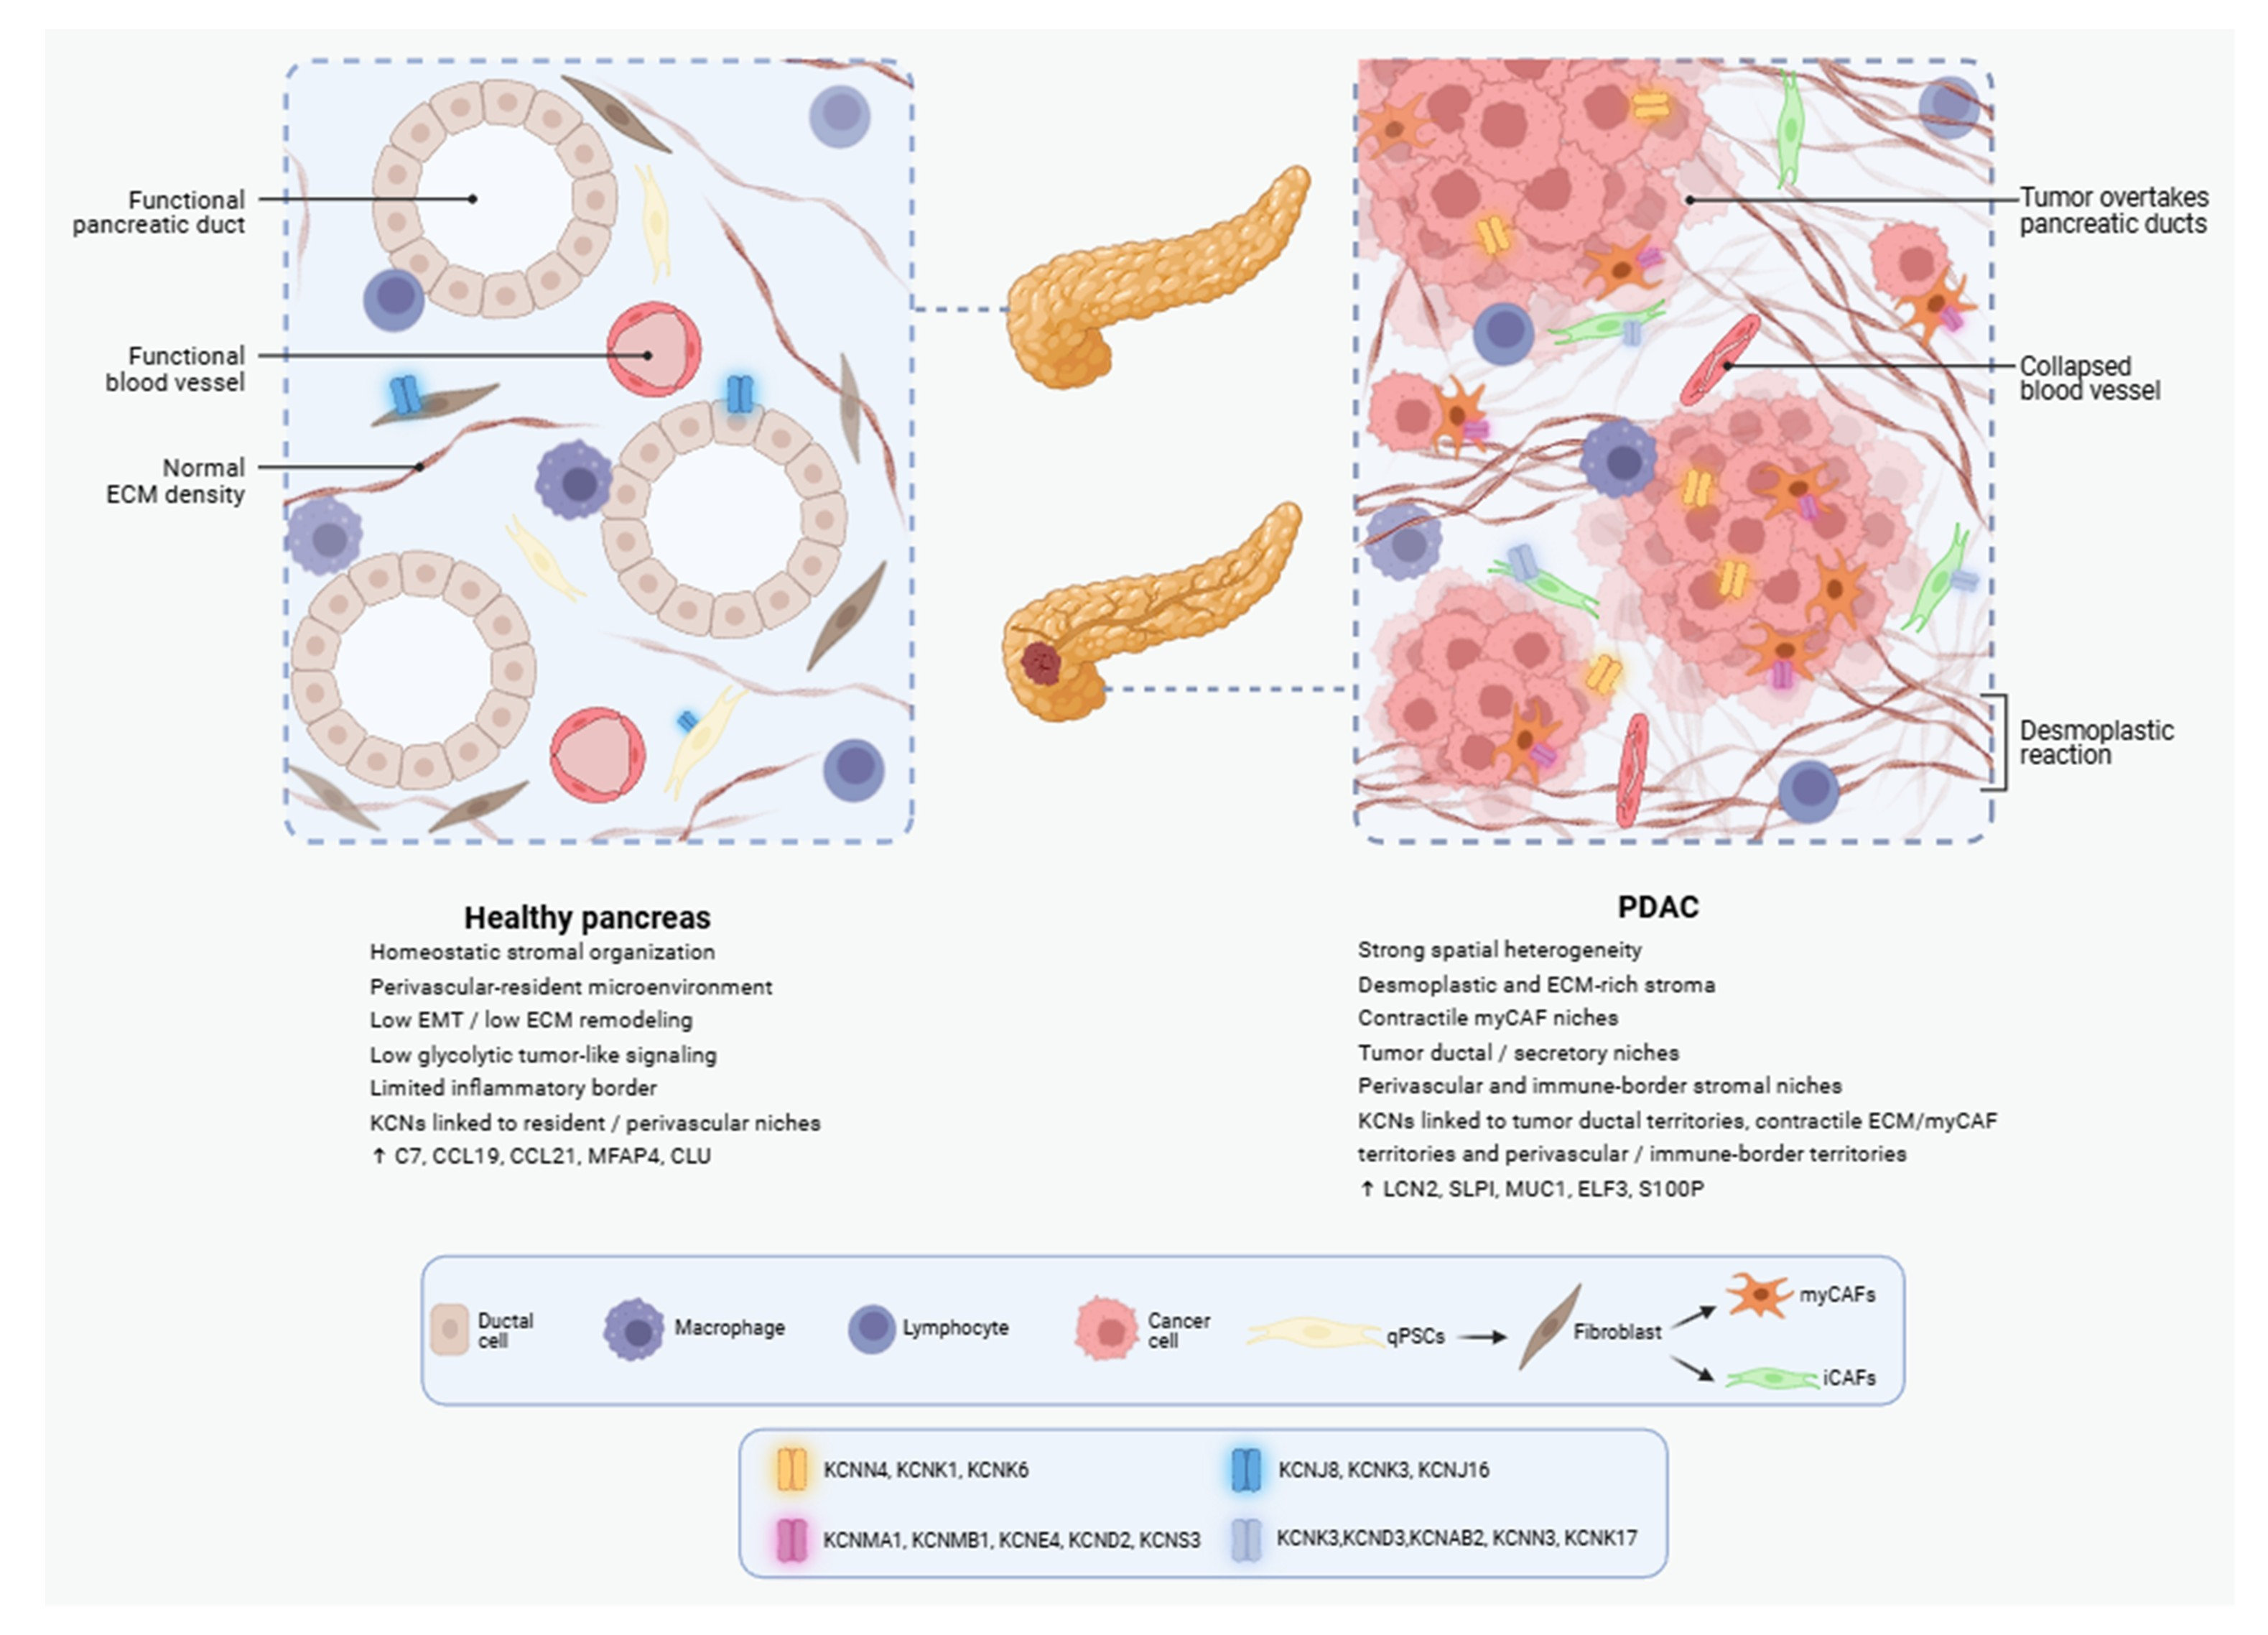
\includegraphics[width=1.05\textwidth]{F7.JPG}}
\caption{\textbf{Summary of the selected KCN landscape in PDAC.} The scheme summarizes the proposed relationship between PDAC stroma, tumor territories, and the main KCN candidates emphasized in this report, with a (simplified) comparison to non-diseased pancreas. The broader KCN union also suggests a directional organization of additional candidates across the PDAC microenvironment.}
\end{figure}

This report used a multi-level bioinformatic workflow to study potassium channel candidates in PDAC stroma. The main result is not the identification of one universal stromal channel, but the definition of a small and interpretable landscape. \textit{KCNMA1} is the strongest candidate for an activated, matrix-rich, and contractile stromal pole. \textit{KCNJ8} supports a more quiescent or resident-like stromal pole. \textit{KCNN4} is the clearest tumor epithelial counterpoint and helps avoid an overly simplified all-stromal interpretation.

This model is coherent because it is supported by complementary data layers. The Moffitt stromal block provides the main stromal polarity. The USER atlas repositions the candidates in a broader tumor microenvironment. The local bulk RNA-seq model shows that BKCa silencing in CAFs is linked to measurable transcriptomic change. The spatial block shows that \textit{KCNMA1} and \textit{KCNN4} do not occupy the same biological territories in tissue.

The iCAF axis remains an important biological question, but it did not yield a KCN candidate as robust as \textit{KCNMA1} or \textit{KCNJ8} in this report. This should be interpreted as a limit of the current datasets and statistical power rather than as a proof that ion channels are irrelevant to iCAF biology.

Future work can extend this study in four directions. First, the current workflow can be formalized (and will be) into a more reusable pipeline for additional ion channel families. Second, the strongest candidates can be tested experimentally in more direct stromal models to determine whether the \textit{KCNMA1}/BKCa axis modulates fibroblast mechanics, matrix deposition, or stromal immune signaling. There is evidence from another fibrotic context, where the BK channel regulatory subunit \textit{KCNMB1} has been linked to myofibroblast differentiation and pulmonary fibrosis \citep{scruggs2020}. In another tumor microenvironment, recent single-cell and spatial analyses of brain metastasis identified a \textit{KCNMA1}-high CAF subcluster within a contractile fibroblast compartment, giving additional support for a stromal and contractile interpretation of \textit{KCNMA1} beyond PDAC \citep{simon2026}. Together with findings linking BK signaling to myofibroblast differentiation in fibrosis \citep{scruggs2020}, this suggests that \textit{KCNMA1} may already be involved in stromal programs in other organs, while remaining relatively unexplored in PDAC. In this context, the results observed here may be consistent with an early indication of a similar stromal role in pancreatic cancer. The laboratory is currently exploring this direction on PDAC. Third, another direction I am currently exploring is MISTy (Multiview Intercellular SpaTial modeling), an interpretable machine-learning method for spatial data that helps separate intrinsic gene-expression patterns from neighborhood and tissue-context effects. I am interested in developing this analysis further to test whether \textit{KCNMA1}, and more broadly the other KCN genes from the union, are mainly associated with stromal cell states or with specific multicellular spatial contexts in PDAC. Fourth, integrating spatial proteomics data would provide an important complement to the transcriptomic analyses presented here, as it would allow the spatial distribution of proteins to be assessed directly and help determine whether the observed transcriptional patterns are reflected at the functional protein level. This perspective is especially interesting because the broader KCN union already suggests a wider organization of potassium channel programs across the PDAC microenvironment.

\phantomsection
\section*{Clinical Opening and Limitations}
\addcontentsline{toc}{section}{Clinical Opening and Limitations}
As a secondary extension, bulk survival analysis was performed to ask whether some prioritized KCN genes also show a clinical signal at patient level. In practice, this part combined a multicohort two-stage Cox meta-analysis and within-cohort Kaplan--Meier exploration. The results were interesting but remained modest. For example, higher \textit{KCNT2} and \textit{KCNMA1} tended to be associated with better outcome, whereas higher \textit{KCNMB4} tended to be associated with worse outcome. However, no KCN remained significant after BH correction in the main meta-analysis, and the direction or strength of the signal could vary across cohorts. This part therefore supports the idea that some stromal or microenvironment KCN may leave a clinical trace, but it remains limited because bulk cohorts cannot resolve stromal localization, cannot separate stromal and tumor contributions directly, and cannot establish mechanism...

\clearpage
\phantomsection
\addcontentsline{toc}{section}{References}
\begin{thebibliography}{99}

\bibitem[DeTomaso and Yosef(2021)]{detomaso2021}
DeTomaso, D., and Yosef, N. (2021). Hotspot identifies informative gene modules and local expression structure in single-cell and spatial transcriptomic data. \textit{Cell Systems}, 12(5), 446--456.

\bibitem[Elyada et al.(2019)]{elyada2019}
Elyada, E., Bolisetty, M., Laise, P., et al. (2019). Cross-species single-cell analysis of pancreatic ductal adenocarcinoma reveals antigen-presenting cancer-associated fibroblasts. \textit{Cancer Discovery}, 9(8), 1102--1123.

\bibitem[Finak et al.(2015)]{finak2015}
Finak, G., McDavid, A., Yajima, M., et al. (2015). MAST: a flexible statistical framework for assessing transcriptional changes and characterizing heterogeneity in single-cell RNA sequencing data. \textit{Genome Biology}, 16, 278.

\bibitem[He et al.(2022)]{he2022}
He, J., Lin, L., and Chen, J. (2022). Practical bioinformatics pipelines for single-cell RNA-seq data analysis. \textit{Biophysics Reports}, 8(3), 158--169.

\bibitem[Hosein et al.(2019)]{hosein2019}
Hosein, A. N., Huang, H., Wang, Z., et al. (2019). Cellular heterogeneity during pancreatic ductal adenocarcinoma progression at single-cell resolution. \textit{JCI Insight}, 5(16), e129212.

\bibitem[Jiang et al.(2019)]{jiang2019}
Jiang, S. H., Zhu, L. L., Zhang, M., et al. (2019). GABRP regulates chemokine signalling, macrophage recruitment and tumour progression in pancreatic cancer through tuning KCNN4-mediated Ca$^{2+}$ signalling in a GABA-independent manner. \textit{Gut}, 68(11), 1994--2006.

\bibitem[Khaliq et al.(2024)]{khaliq2024}
Khaliq, A. M., Erdogan, C., Kurt, Z., et al. (2024). Integrated spatial transcriptomics reveals multicellular ecotypes in pancreatic cancer. \textit{Nature Genetics}, 56, 423--435.

\bibitem[Korotkevich et al.(2021)]{korotkevich2021}
Korotkevich, G., Sukhov, V., Budin, N., et al. (2021). Fast gene set enrichment analysis. \textit{bioRxiv}. doi:10.1101/060012.

\bibitem[Luecken and Theis(2019)]{luecken2019}
Luecken, M. D., and Theis, F. J. (2019). Current best practices in single-cell RNA-seq analysis: a tutorial. \textit{Molecular Systems Biology}, 15(6), e8746.

\bibitem[Love et al.(2014)]{love2014}
Love, M. I., Huber, W., and Anders, S. (2014). Moderated estimation of fold change and dispersion for RNA-seq data with DESeq2. \textit{Genome Biology}, 15, 550.

\bibitem[Oh et al.(2023)]{oh2023}
Oh, S., et al. (2023). Coordinated single-cell tumor microenvironment dynamics reinforce pancreatic cancer subtype. \textit{Nature Communications}, 14, 4352.

\bibitem[Ohlund et al.(2017)]{ohlund2017}
Ohlund, D., Handly-Santana, A., Biffi, G., et al. (2017). Distinct populations of inflammatory fibroblasts and myofibroblasts in pancreatic cancer. \textit{Journal of Experimental Medicine}, 214(3), 579--596.

\bibitem[Hwang et al.(2020)]{peng2020}
Hwang, W. L., Jagadeesh, K. A., Guo, J. A., et al. (2020). Single-nucleus and spatial transcriptomics of archival pancreatic cancer reveals multi-compartment reprogramming after neoadjuvant treatment. \textit{bioRxiv}. doi:10.1101/2020.08.25.267336.

\bibitem[Rapetti-Mauss et al.(2023)]{rapetti2023}
Rapetti-Mauss, R., Nigri, J., Berenguier, C., et al. (2023). SK2 channels set a signalling hub bolstering CAF-triggered tumourigenic processes in pancreatic cancer. \textit{Gut}, 72, 722--735.

\bibitem[Scruggs et al.(2020)]{scruggs2020}
Scruggs, A. M., et al. (2020). The role of KCNMB1 and BK channels in myofibroblast differentiation and pulmonary fibrosis. \textit{American Journal of Respiratory Cell and Molecular Biology}, 62(2), 191--203.

\bibitem[Simon et al.(2026)]{simon2026}
Simon, T., Buckley, D. N., Yang, Z., Matsuba, C., Tew, B. Y., Gooden, G. C., Hurth, K., Toms, S. A., Tran, D. D., Zada, G., Salomon, M. P., and Salhia, B. (2026). Single cell and spatial sequencing analysis of cancer associated fibroblasts in the brain metastasis tumor microenvironment. \textit{Communications Biology}. https://doi.org/10.1038/s42003-026-09915-1.

\bibitem[Subramanian et al.(2005)]{subramanian2005}
Subramanian, A., Tamayo, P., Mootha, V. K., et al. (2005). Gene set enrichment analysis: a knowledge-based approach for interpreting genome-wide expression profiles. \textit{Proceedings of the National Academy of Sciences of the United States of America}, 102(43), 15545--15550.

\bibitem[Vieth et al.(2019)]{vieth2019}
Vieth, B., Parekh, S., Ziegenhain, C., et al. (2019). A systematic evaluation of single cell RNA-seq analysis pipelines. \textit{Nature Communications}, 10, 4667.

\end{thebibliography}

\clearpage
\phantomsection
\section*{M1 Skills Summary}
\addcontentsline{toc}{section}{M1 Skills Summary}
During this internship, I learned how to organize a multi-level bioinformatic workflow, work with scRNA-seq, snRNA-seq, bulk RNA-seq, and spatial transcriptomic datasets, perform patient-aware pseudobulk analyses, and connect pathway enrichment results to an interpretable biological model. I also improved my ability to document analytical steps, generate readable figures, and discuss transcriptomic results with the level of caution required for low-abundance genes such as ion channels.
More than just technical skills, this project showed me how exciting and complex cancer biology is when studied through bioinformatics. I learned that data analysis is about asking the right statistical questions, searching for the proper tools, and staying critical of the results. It requires a lot of trial and error, trying again and again even when things do not work or look blurry at first, and remaining calm to find the answers (at least, try to get some). So it taught me how to make "important" choices, justify them, and never stop questioning the data.
I also improved my ability to communicate bioinformatic results with biologists, and to explain statistical or computational methods in simple terms so that they remained understandable and useful in discussion. Presenting my work during lab meetings also helped me gain confidence in speaking about data, defending analytical choices, and adapting explanations to different scientific backgrounds.
Another important aspect of this internship was the motivation that comes from working on a concrete project in a laboratory environment. Seeing analyses become part of an active research question made the work much more meaningful and rewarding. It also showed me that many concepts learned during the Master's program, especially in omics and statistics, were directly useful in practice and really helped me move forward in this project.
This internship reassured me that I made the right choice in following this path. It confirmed how much I enjoy bioinformatics, cancer-related questions, and molecular biology, showed me how much I still have to learn, and made me look forward even more to what comes next !

\clearpage
\phantomsection
\section*{Seminar Attendance Sheet}
\addcontentsline{toc}{section}{Seminar Attendance Sheet}
\begin{figure}[H]
\centering
\makebox[\textwidth][c]{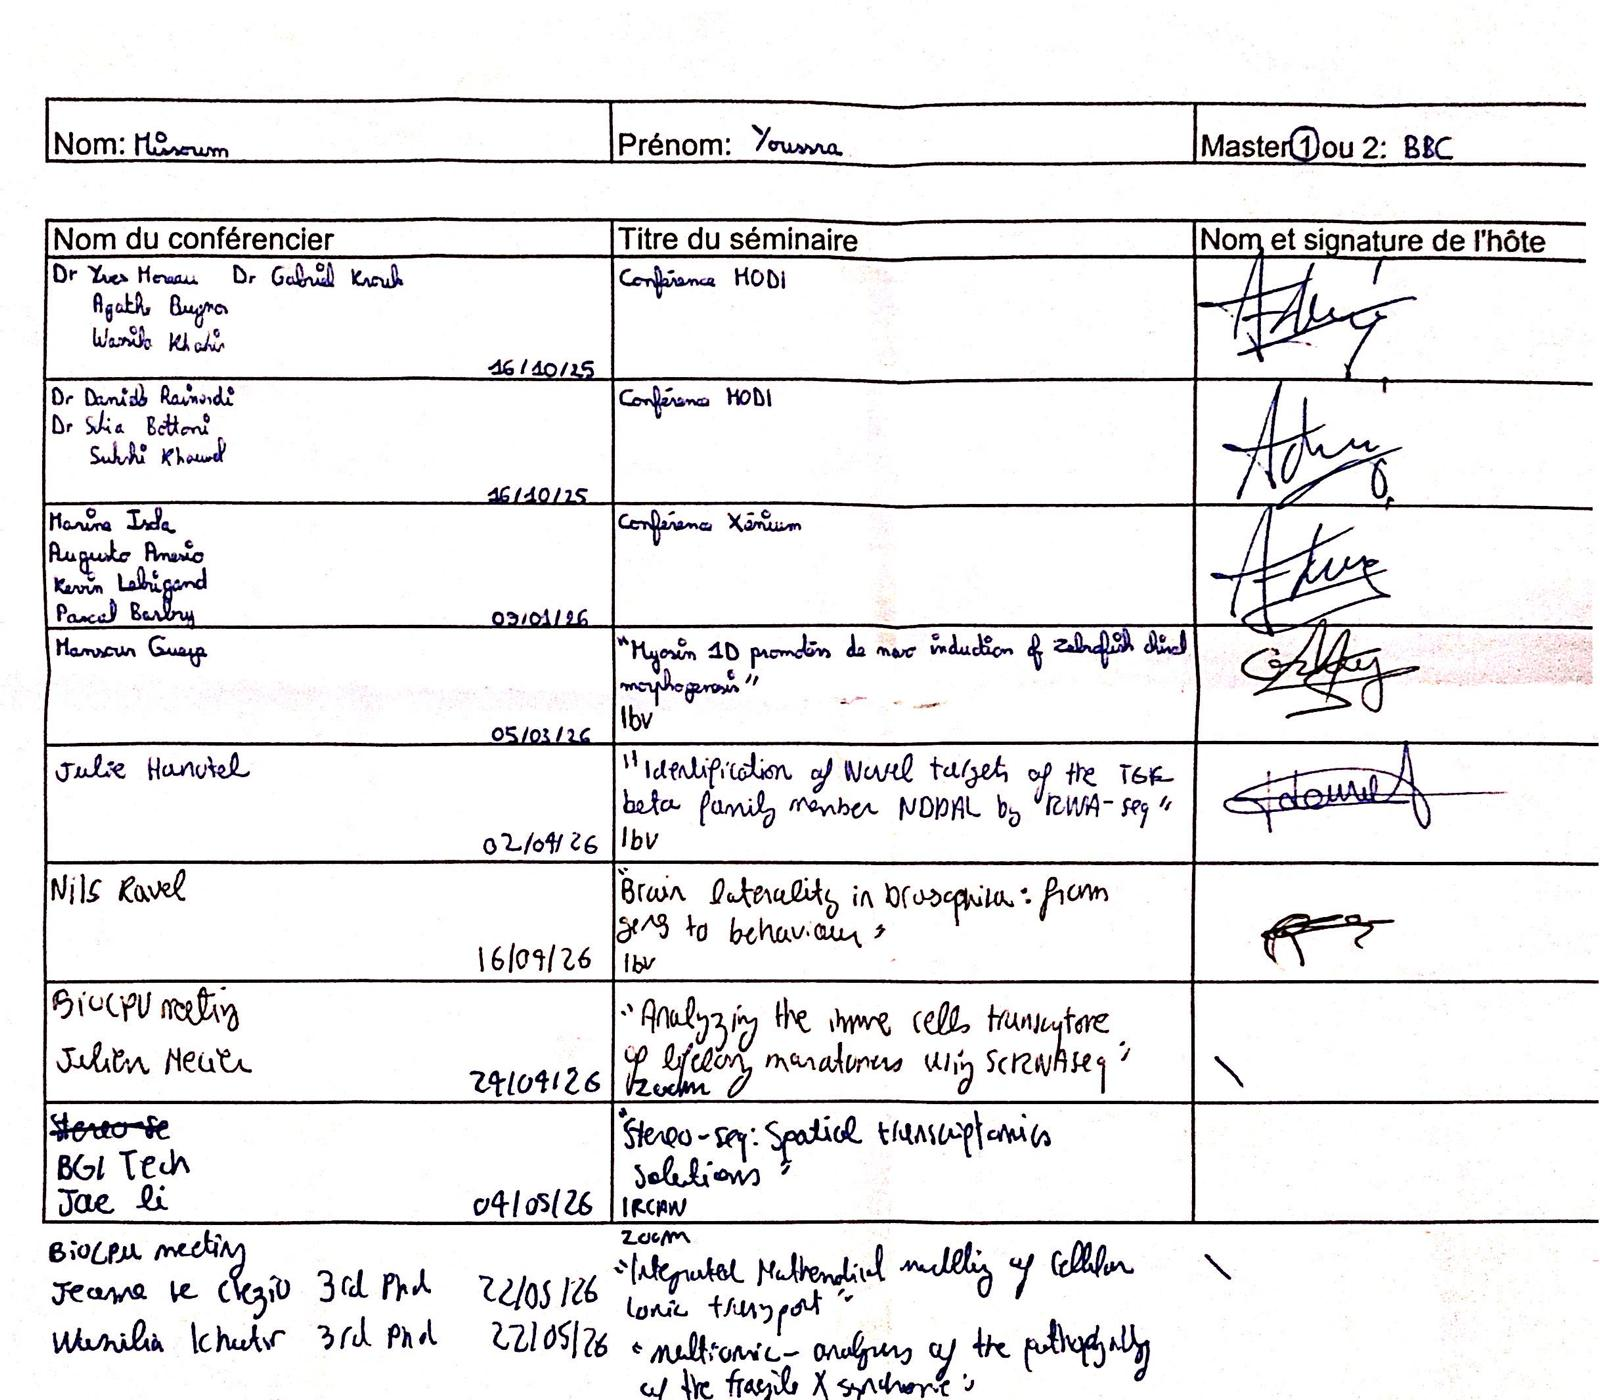
\includegraphics[width=0.9\textwidth]{seminar_attendance.jpg}}
\end{figure}

\end{document}
